\documentclass[hidelinks]{article}
\title{A Novel Statistical Framework To Jointly Model Genetic and Epigenetic Regulation of Tissue-Specific Gene Expression}
\author{Chaitanya~R. Acharya, Kouros Owzar and Andrew~S. Allen}
\date{\today}

\usepackage[center]{caption}
\usepackage{bm}
\usepackage{amsmath}
\usepackage{amssymb}
\usepackage{amsbsy}
\usepackage{amsfonts}
\usepackage{amscd}
\usepackage{ifthen}
\usepackage[utf8]{inputenc}
\usepackage{graphicx}
\usepackage{subfigure}
\usepackage{hyperref}
\usepackage{float}
\restylefloat{figure,table}
\usepackage{array}
\usepackage{longtable}
\usepackage{pdflscape}
%\setlength\LTleft{0pt}
%\setlength\LTright{0pt}
%\usepackage{pgfplots}
%\usepackage{pgfplotstable}
%\pgfplotsset{compat=newest}
%\usepackage[landscape]{geometry}
\usepackage{colortbl}
\usepackage{courier}
\usepackage{verbatim}
\usepackage{relsize,setspace}
\usepackage{tabularx,ragged2e,booktabs}
\usepackage{multicol}
%\usepackage{Sweave}
\usepackage{empheq}
%\SweaveOpts{keep.source=F, concordance=T, height=5, width=10}
\usepackage{fancyhdr}
\pagestyle{fancyplain}
\fancyhf{}
\lhead{\fancyplain{}{}}
\rhead{\fancyplain{}{\today}}
\rfoot{\fancyplain{}{\thepage}}
\lfoot[\thepage]{}
\rfoot[]{\thepage}
\newcommand{\code}[1]{\texttt{\smaller #1}}
\newcommand{\R}{{\normalfont\textsf{R}}{}}
\parskip 1.25ex
\parindent 0ex
\textwidth 6.75in
\textheight 9.25in
\topmargin -.875in
\oddsidemargin -.125in
\evensidemargin -.125in  
\usepackage{multirow}
\usepackage{hhline}
\usepackage{color}
\usepackage{listings}
\usepackage[table]{xcolor}
\usepackage{textcomp}
\usepackage{breqn}
\usepackage{arydshln}
\definecolor{listinggray}{gray}{0.9}
\definecolor{lbcolor}{rgb}{0.9,0.9,0.9}
\usepackage{soul}
\usepackage{booktabs}% http://ctan.org/pkg/booktabs
\newcommand{\tabitem}{~~\llap{\textbullet}~~}
%% alternate rowcolors for all tables
%\let\oldtabular\tabular
%\let\endoldtabular\endtabular
%\renewenvironment{tabular}{\rowcolors{2}{white}{lightgray}\oldtabular}{\endoldtabular}

%% alternate rowcolors for all long-tables
%\let\oldlongtable\longtable
%\let\endoldlongtable\endlongtable
%\renewenvironment{longtable}{\rowcolors{2}{white}{lightgray}\oldlongtable} {
%\endoldlongtable}

\DeclareMathOperator{\Tr}{Tr}

\newcolumntype{x}[1]{%
>{\centering\hspace{0pt}}p{#1}}%
                                             
\setkeys{Gin}{width=0.70 \textwidth} 		

\newcommand{\fig}[1]{\centerline{\includegraphics{#1}}}

\DeclareGraphicsExtensions{.pdf, .jpg, .png}

\usepackage{tikz}
\usetikzlibrary{shapes,arrows,chains,decorations.pathmorphing,decorations.pathreplacing,matrix,backgrounds}
\tikzstyle{block1} = [rectangle, sharp corners, draw, text width=5em, 
                     text centered, fill=red!20,
                     minimum height=1em, node distance=4cm]
\tikzstyle{block2} = [rectangle, sharp corners, draw, text width=5em, 
                     text centered, fill=black!20, minimum width=1mm,
                     minimum height=1em, node distance= 4cm]
\tikzstyle{block3} = [rectangle, sharp corners, draw, text width=1em, 
                     text centered, fill=black, minimum width=1mm,
                     minimum height=1em, node distance= 4cm]
                     
\tikzstyle{line} = [draw, very thick,-latex']
\tikzstyle{dline} = [draw, very thick,dashed,-latex']

\tikzstyle{block} = [rectangle, draw, text width=5em, 
                     text centered, rounded corners, fill=blue!20,
                     minimum height=4em, node distance=4cm]
\tikzstyle{line} = [draw, very thick,-latex']
\tikzstyle{dline} = [draw, very thick,dashed,-latex']
\begin{document}
\maketitle

\tableofcontents
\listoffigures
\setcounter{tocdepth}{3}

\section{Background \& Motivation}

\begin{figure}[H]
\begin{center}
\resizebox{8.0cm}{!}{%
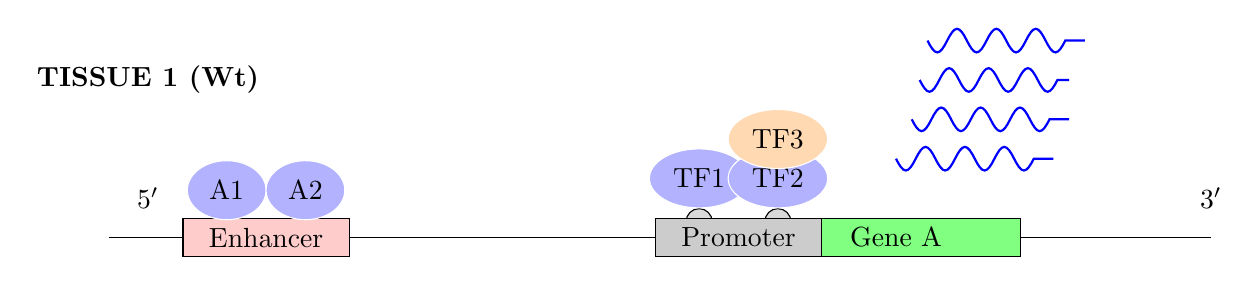
\begin{tikzpicture}[decoration={coil}, dna/.style={decorate, thick, decoration={aspect=0, segment length=0.5cm}}, protein/.style={ellipse, draw=white, minimum width=1cm, minimum height=1cm},
gluon/.style={decorate, thick, decoration={aspect=0, segment length=0.5cm}},cpg/.style={circle, draw=black, minimum width=1mm, minimum height=1mm}]
%DNA
%\draw[dna, decoration={amplitude=.15cm}] (.1,0) -- (14,0);
%\draw[dna, decoration={amplitude=-.15cm}] (0,0) -- (14,0);
\draw(0,0) -- (14,0);
 %Gene
\node[block1,sharp corners, fill=green!50, inner xsep=20pt] at (10,0) (gene){Gene A};
\draw[gluon,blue,decoration={amplitude=-.15cm}] (10,1) -- (12,1) ;
\draw[gluon,blue,decoration={amplitude=-.15cm}] (10.2,1.5) -- (12.2,1.5) ;
\draw[gluon,blue,decoration={amplitude=-.15cm}] (10.3,2) -- (12.2,2) ;
\draw[gluon,blue,decoration={amplitude=-.15cm}] (10.4,2.5) -- (12.4,2.5) ;

% CpG
\node[cpg,minimum height=2.5mm,fill=gray!30] at (7.5,0.2){};
\node[cpg,minimum height=2.5mm,fill=gray!30] at (8.5,0.2){};

%Promoter
\node[block1,inner xsep=5pt] at (2,0) (box1){Enhancer};
%\node[block3,inner xsep=0.5pt] at (4,0) (box2){ };
%\node[block3,inner xsep=0.5pt] at (5,0) (box3){ };
\node[block2,sharp corners, inner xsep=5pt] at (8,0) (box4){Promoter};
%\draw [decorate,decoration={brace,amplitude=10pt},rotate=+90] (-1,-1) -- (-1,-9.0);
%\draw [decorate,decoration={brace,mirror,amplitude=10pt},rotate=+90] (-0.5,-0.5) -- (-0.5,-9.0);
%\node (RR) at (5,-1.5) {Regulatory region};

% Proteins
\node [protein, minimum height=.75cm,fill=blue!30] at (1.5,0.6) {A1};
\node [protein, minimum height=.75cm,fill=blue!30] at (2.5,0.6) {A2};

\node [protein, minimum height=.75cm,fill=blue!30] at (7.5,0.75) {TF1};
\node [protein, minimum height=.75cm,fill=blue!30] at (8.5,0.75) {TF2};
\node [protein, minimum height=.75cm,fill=orange!30] at (8.5,1.25) {TF3};


\node (5p) at (0.5,0.5) {$5^\prime$};
\node (3p) at (14,0.5) {$3^\prime$};
\node (tissue1) at (0.5,2) {\textbf{TISSUE 1 (Wt) }};
\end{tikzpicture}
}
\vspace{1cm}
\resizebox{8.0cm}{!}{%
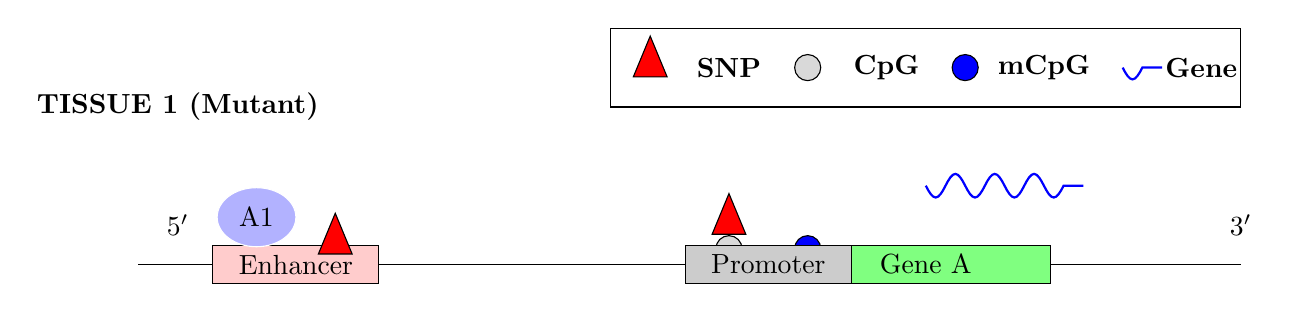
\begin{tikzpicture}[decoration={coil},
dna/.style={decorate, thick, decoration={aspect=0, segment length=0.5cm}},
protein/.style={ellipse, draw=white, minimum width=1cm, minimum height=1cm},
gluon/.style={decorate, thick, decoration={aspect=0, segment length=0.5cm}},
cpg/.style={circle, draw=black, minimum width=1mm, minimum height=1mm}] 
%DNA
%\draw[dna, decoration={amplitude=.15cm}] (.1,0) -- (14,0);
%\draw[dna, decoration={amplitude=-.15cm}] (0,0) -- (14,0);
\draw(0,0) -- (14,0);
 %Gene
\node [block1,sharp corners, fill=green!50, inner xsep=20pt] at (10,0) (gene){Gene A};
\draw[gluon,blue,decoration={amplitude=-.15cm}] (10,1) -- (12,1) ;
% CpG
\node[cpg,minimum height=2.5mm,fill=gray!30] at (7.5,0.2){};
\node[cpg,minimum height=2.5mm,fill=blue] at (8.5,0.2){};

%Promoter
\node[block1,inner xsep=5pt] at (2,0) (box1){Enhancer};
%\node[block3,inner xsep=0.5pt] at (4,0) (box2){ };
%\node[block3,inner xsep=0.5pt] at (5,0) (box3){ };
%\node[block3,inner xsep=0.5pt] at (5.5,0) (box3.1){ };
\node[block2,sharp corners, inner xsep=5pt] at (8,0) (box4){Promoter};
\node at (2.5,0.25)[isosceles triangle, fill=red,draw=black,rotate=90,minimum size=0.25mm,minimum height=0.25mm](SNP){};
\node at (7.5,0.5)[isosceles triangle, fill=red,draw=black,rotate=90,minimum size=0.25mm,minimum height=0.25mm](SNP1){};
%\draw [decorate,decoration={brace,mirror,amplitude=10pt},rotate=+90] (-0.5,-0.5) -- (-0.5,-9.0);
%\node (RR) at (2.5,1.5) {SNP};
%\draw[->](RR)--(SNP);
% Proteins
\node [protein, minimum height=.75cm,fill=blue!30] at (1.5,0.6) {A1};
%\node [protein, minimum height=.75cm,fill=blue!30] at (2.5,0.6) {A2};

%\node [protein, minimum height=.75cm,fill=blue!30] at (7.5,0.75) {TF1};
%\node [protein, minimum height=.75cm,fill=blue!30] at (8.5,0.75) {TF2};
%\node [protein, minimum height=.75cm,fill=orange!30] at (8.5,1.25) {TF3};

\node (5p) at (0.5,0.5) {$5^\prime$};
\node (3p) at (14,0.5) {$3^\prime$};
\node (tissue11) at (0.5,2) {\textbf{TISSUE 1 (Mutant) }};

% Legend
\node at (6.5,2.5)[isosceles triangle, fill=red,draw=black,rotate=90,minimum size=0.25mm,minimum height=0.25mm](SNP2){};
\node(legend1) at (7.5,2.5){\textbf{SNP}};
\node[cpg,minimum height=2.5mm,fill=gray!30] at (8.5,2.5){};
\node(legend2) at (9.5,2.5){\textbf{CpG }};
\node[cpg,minimum height=2.5mm,fill=blue] at (10.5,2.5){};
\node(legend3) at (11.5,2.5){\textbf{mCpG }};
\draw[gluon,blue,decoration={amplitude=-.15cm}] (12.5,2.5) -- (13,2.5) ;
\node(legend4) at (13.5,2.5){\textbf{Gene }};
\draw (6,3)--(14,3)--(14,2)--(6,2)--(6,3);
\end{tikzpicture}
}
\resizebox{8cm}{!}{%
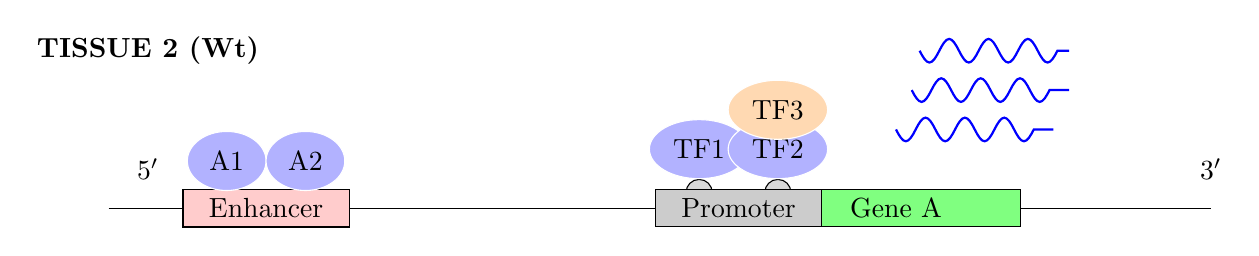
\begin{tikzpicture}[decoration={coil},
dna/.style={decorate, thick, decoration={aspect=0, segment length=0.5cm}},
protein/.style={ellipse, draw=white, minimum width=1cm, minimum height=1cm},
gluon/.style={decorate, thick, decoration={aspect=0, segment length=0.5cm}},
cpg/.style={circle, draw=black, minimum width=1mm, minimum height=1mm}] 
%DNA
%\draw[dna, decoration={amplitude=.15cm}] (.1,0) -- (14,0);
%\draw[dna, decoration={amplitude=-.15cm}] (0,0) -- (14,0);
\draw(0,0) -- (14,0);
 %Gene
\node [block1,sharp corners, fill=green!50, inner xsep=20pt] at (10,0) (gene){Gene A};
\draw[gluon,blue,decoration={amplitude=-.15cm}] (10,1) -- (12,1) ;
\draw[gluon,blue,decoration={amplitude=-.15cm}] (10.2,1.5) -- (12.2,1.5) ;
\draw[gluon,blue,decoration={amplitude=-.15cm}] (10.3,2) -- (12.2,2) ;

% CpG
\node[cpg,minimum height=2.5mm,fill=gray!30] at (7.5,0.2){};
\node[cpg,minimum height=2.5mm,fill=gray!30] at (8.5,0.2){};

%Promoter
\node[block1,inner xsep=5pt] at (2,0) (box1){Enhancer};
%\node[block3,inner xsep=0.5pt] at (4,0) (box2){ };
%\node[block3,inner xsep=0.5pt] at (5,0) (box3){ };
%\node[block3,inner xsep=0.5pt] at (5.5,0) (box3.1){ };
\node[block2,sharp corners, inner xsep=5pt] at (8,0) (box4){Promoter};
%\draw [decorate,decoration={brace,amplitude=10pt},rotate=+90] (1,1) -- (1,9);
%\draw [decorate,decoration={brace,mirror,amplitude=10pt},rotate=+90] (-0.5,-0.5) -- (-0.5,-9.0);
%\node (RR) at (5,-1.5) {Regulatory region};

% Proteins
\node [protein, minimum height=.75cm,fill=blue!30] at (1.5,0.6) {A1};
\node [protein, minimum height=.75cm,fill=blue!30] at (2.5,0.6) {A2};

\node [protein, minimum height=.75cm,fill=blue!30] at (7.5,0.75) {TF1};
\node [protein, minimum height=.75cm,fill=blue!30] at (8.5,0.75) {TF2};
\node [protein, minimum height=.75cm,fill=orange!30] at (8.5,1.25) {TF3};

\node (5p) at (0.5,0.5) {$5^\prime$};
\node (3p) at (14,0.5) {$3^\prime$};
\node (tissue2) at (0.5,2) {\textbf{TISSUE 2 (Wt)}};
%\node (wt) at (14,2) {\textbf{Wild type}};
\end{tikzpicture}
}
\resizebox{8.0cm}{!}{%
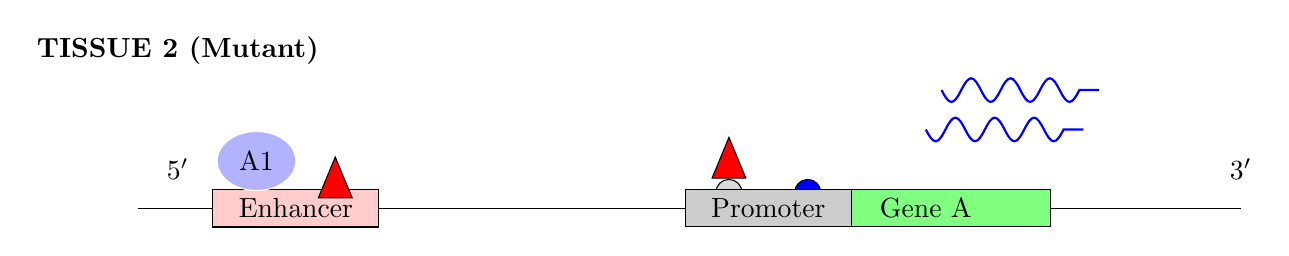
\begin{tikzpicture}[decoration={coil},
dna/.style={decorate, thick, decoration={aspect=0, segment length=0.5cm}},
protein/.style={ellipse, draw=white, minimum width=1cm, minimum height=1cm},
gluon/.style={decorate, thick, decoration={aspect=0, segment length=0.5cm}},
cpg/.style={circle, draw=black, minimum width=1mm, minimum height=1mm}] 
%DNA
%\draw[dna, decoration={amplitude=.15cm}] (.1,0) -- (14,0);
%\draw[dna, decoration={amplitude=-.15cm}] (0,0) -- (14,0);
\draw(0,0) -- (14,0);

 %Gene
\node [block1,sharp corners, fill=green!50, inner xsep=20pt] at (10,0) (gene){Gene A};
\draw[gluon,blue,decoration={amplitude=-.15cm}] (10,1) -- (12,1) ;
\draw[gluon,blue,decoration={amplitude=-.15cm}] (10.2,1.5) -- (12.2,1.5) ;

% CpG
\node[cpg,minimum height=2.5mm,fill=gray!30] at (7.5,0.2){};
\node[cpg,minimum height=2.5mm,fill=blue] at (8.5,0.2){};

%Promoter
\node[block1,inner xsep=5pt] at (2,0) (box1){Enhancer};
%\node[block3,inner xsep=0.5pt] at (4,0) (box2){ };
%\node[block3,inner xsep=0.5pt] at (5,0) (box3){ };
%\node[block3,inner xsep=0.5pt] at (5.5,0) (box3.1){ };
\node[block2,sharp corners, inner xsep=5pt] at (8,0) (box4){Promoter};
\node at (2.5,0.25)[isosceles triangle, fill=red,draw=black,rotate=90,minimum size=0.25mm,minimum height=0.25mm](SNP){};
\node at (7.5,0.5)[isosceles triangle, fill=red,draw=black,rotate=90,minimum size=0.25mm,minimum height=0.25mm](SNP1){};
%\draw [decorate,decoration={brace,mirror,amplitude=10pt},rotate=+90] (-0.5,-0.5) -- (-0.5,-9.0);
%\node (RR) at (2.5,1.5) {SNP};
%\draw[->](RR)--(SNP);
% Proteins
\node [protein, minimum height=.75cm,fill=blue!30] at (1.5,0.6) {A1};
%\node [protein, minimum height=.75cm,fill=blue!30] at (2.5,0.6) {A2};

%\node [protein, minimum height=.75cm,fill=blue!30] at (7.5,0.75) {TF1};
%\node [protein, minimum height=.75cm,fill=blue!30] at (8.5,0.75) {TF2};
%\node [protein, minimum height=.75cm,fill=orange!30] at (8.5,1.25) {TF3};

\node (5p) at (0.5,0.5) {$5^\prime$};
\node (3p) at (14,0.5) {$3^\prime$};
%\node (tissue2) at (0.5,2) {\textbf{Tissue 2}};
%\draw [decorate,decoration={brace,mirror,amplitude=10pt}] (-0.5,-0.5) -- (-0.5,-9.0);
\node (tissue21) at (0.5,2) {\textbf{TISSUE 2 (Mutant)}};
\end{tikzpicture}
}
\end{center}
\label{Figure}
\caption[Epigenetic and genetic regulation of tissue-specific gene expression - a concept figure]{An illustration of tissue-specific gene expression of Gene A (quantified by blue squiggly lines) and the effect of the same genetic variant (denoted by red triangle labeled SNP) and the methylation status of the proximal CpG island (denoted by shaded semi-circle) in its expression in tissues 1 and 2}
\end{figure}

It has been long established that regulatory regions in higher eukaryotes activate gene transcription in a tissue-specific manner \cite{enhancer,geyer}. These regulatory regions are susceptible to both genetic variation and epigenetic modifications that play a coordinated role in regulating tissue-specific gene expression \cite{JTBell, gibbs, shoemaker, wrzodek,epigen_reg}. One form of epigenetic variation is DNA methylation that targets non-methylated CpG sites, which constitute approximately 70\% of all annotated promoters \cite{cpg}. DNA methylation is linked to transcriptional silencing, and many CpG island promoters are active in a tissue-specific manner. Previous studies have shown that genetic variants at CpG sites are likely to disrupt DNA methylation and thus drastically change the methylation status at a single CpG site \cite{wagner,hellman,gen_epigen_tissue}. Since an increased DNA methylation at any of the CpG sites located in either the promoter or the intronic regions leads to a decreased gene expression, any variation in the CpG sites could lead to an opposite effect. For example, Catechol-O -methyltransferase (COMT) gene, which is implicated in schizophrenia has a functional single nucleotide polymorphism (SNP), $Val^{158}$ $Met$ (rs4680) that is associated with differential COMT expression across regions of the brain during the course of the illness \cite{comt1}. More specifically, the substitution of a methionine (Met) for a valine (Val) at position 158 results in reduced activity of the COMT enzyme due to reduced protein stability. Besides the environmental stressors, methylation of CpG islands associated with the aforementioned variant seem to affect the expression of COMT across different brain regions\cite{comt1}. Identifying and studying the mechanisms through which genetic variation, DNA methylation and gene expression interact may provide us with yet another clue to understanding complex phenotypes. 

Genetic control of gene expression can be defined in terms of SNPs and their associations with gene expression. Expression quantitative trait loci (eQTL) are correlations between SNPs and gene expression.  Similarly, epigenetic control of gene expression can be defined in terms of CpG island methylation and their interactions with SNPs. Expression quantitative trait methylations (eQTM) are correlations between gene expression and methylation while methylation quantitative trait loci (mQTL) are correlations between SNPs and methylation. Current approaches involve performing independent eQTL and mQTL analyses within each tissue followed by identifying pairs of statistically significant CpG-SNP and mRNA-SNP \cite{gibbs,gen_epigen_tissue}. These pairs are then expanded to  triplets of SNP and CpG-mRNA pair where the SNP was significantly correlated with either mRNA or CpG site of the CpG-mRNA pair. However, such an approach fails to fully exploit expression patterns across the tissues either by pooling information when a variant has a similar effect across multiple tissues or by explicitly identifying effects that differ across tissues. Even if we identify a variant that effects gene expression of a gene in a given tissue, it is not clear whether the effect is either due to an interaction effect between the genotype and tissue or an interaction effect between genotype, methylation status of a CpG site and tissues. 

%For example, a genetic variant rs3762555 confers a significantly lower methylation at CpG sites in the promoter region of Glutamate decarboxylases (GAD1/GAD2), which play an important role in the pathogenesis of schizophrenia \cite{gad1}. This SNP effect is observed predominantly in the prefrontal cortex region of the brain indicating the region-specificity of interaction between the SNP, CpG site and the gene expression \cite{gad2}. 

We propose a score test-based approach that explicitly models the aforementioned interactions among genotypes, methylation status and tissues as random effects. Our approach does not require parameter estimation under the alternative hypothesis, thus making it computationally tractable. Further, our score-based approach only requires estimation of first two moments of the random effects and, as a result, is robust to misspecification of the random effect distribution. We show using simulations that our joint score test approach is better than a region-by-region (TBT) approach. 

We demonstrate the effectiveness of our method by applying it to a publicly available expression and methylation dataset from adult normal brains and show that by jointly analyzing multiple brain regions (tissues), we identify more mRNA-CpG-SNP triplets relative to a TBT analysis.

\section{Our model}

\begin{figure}[H]
\centering
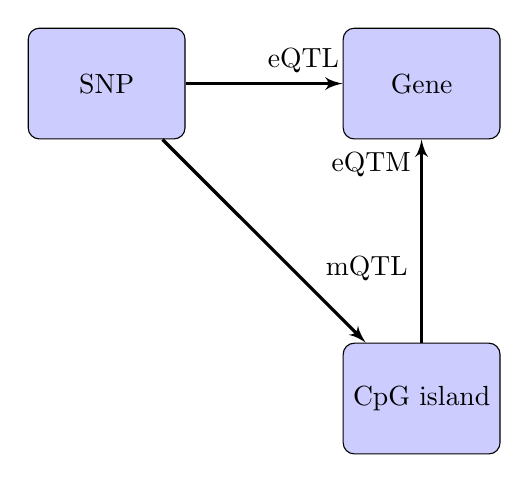
\begin{tikzpicture}[node distance = 3cm, auto]
\node [block] (snp) {SNP};
\node[block, right of=snp] (gene) {Gene};
\node [block, below of=gene] (meth) {CpG island};

\path [line] (snp) -- node [near end] {eQTL} (gene);
\path [line] (snp) --  node [near end] {mQTL} (meth);
\path [line] (meth) -- node[very near end] {eQTM} (gene);

\end{tikzpicture}
\caption[Relationships between mRNA, CpG and SNP]{Tissue-specific gene expression is controlled by genetic, epigenetic and transcriptional regulatory mechanisms. Genetic control of gene expression can be defined in terms of SNPs and their associations with gene expression. Expression quantitative trait loci (eQTL) are correlations between SNPs and gene expression.  Similarly, epigenetic control of gene expression can be defined in terms of CpG island methylation and their interactions with SNPs. Expression quantitative trait methylations (eQTM) are correlations between gene expression and methylation while methylation quantitative trait loci (mQTL) are correlations between SNPs and methylation. Gene expression can be modeled as a function of SNP and CpG islands (if all the requisite data types are available).} 
\label{fig1}
\end{figure}

%\noindent\fbox{%
%    \parbox{\textwidth}{%
%	\textbf{OBJECTIVE:} \newline
%	Leveraging all available genomic information (in this case, CpG island methylation patterns and genotype data) to efficiently identify tissue-specific eQTL. 
%     }%
%}
%
%
%Available data types --
%\begin{enumerate}
%\item Gene expression data
%\item SNP (as GWAS data)
%\item Methylation data 
%\end{enumerate}

For a given gene-SNP pair, gene expression is modeled as a function of genotype and methylation -

\begin{equation}
\large
Y = J\alpha + G\beta + M\lambda + MG\phi + Au + Bv + Cw + Dx + \xi
\end{equation}

where $Y$ is a $nt$-dimensional vector of expression levels in $t$ tissues and $n$ individuals, $\alpha$ is a vector of tissue-specific intercepts, $G$ is a $nt$-dimensional vector of genotypes, $\beta$ is a fixed effect of genotype across tissue, $\lambda$ is an overall methylation-specific fixed effect, $\phi$ is genotype $\times$ methylation interaction effect (fixed effect), $u \sim N\left(0, \tau AA^T \right)$ is a vector of subject-specific random effect, $v \sim N\left(0,\gamma BB^T \right)$ is a vector of tissue-specific random effects, $w \sim N\left(0,\delta CC^T \right)$  is a vector of tissue-specific random effects that describe the interaction effect between genotype and methylation is a vector of random effects describing the interaction between genotype, methylation and tissue, $x \sim N\left(0,\theta DD^T \right)$ is a vector of tissue-specific random effects describing methylation effects and $\xi \sim N\left(0, \epsilon I_{nt} \right)$. The matrices $J$, $A$, $B$, $C$, and $D$ are design matrices with $B$ being a function of genotype, $C$ is a function of both genotype and methylation data and finally, $D$ is a function of just the methylation data. $J$ is $nt \times t$ dimensional matrix denoting the design matrix for the tissue-specific intercepts. $A$ is $nt \times nt$ design matrix for the subject-specific intercepts. $B$ is a $nt \times t$ design matrix of stacked genotypes. $C$ is a $nt \times t$ design matrix of stacked (product of) tissue-specific methylation and genotype data. $D$ is $nt \times t$ design matrices of stacked tissue-specific methylation data. 

\begin{figure}[H]
\centering
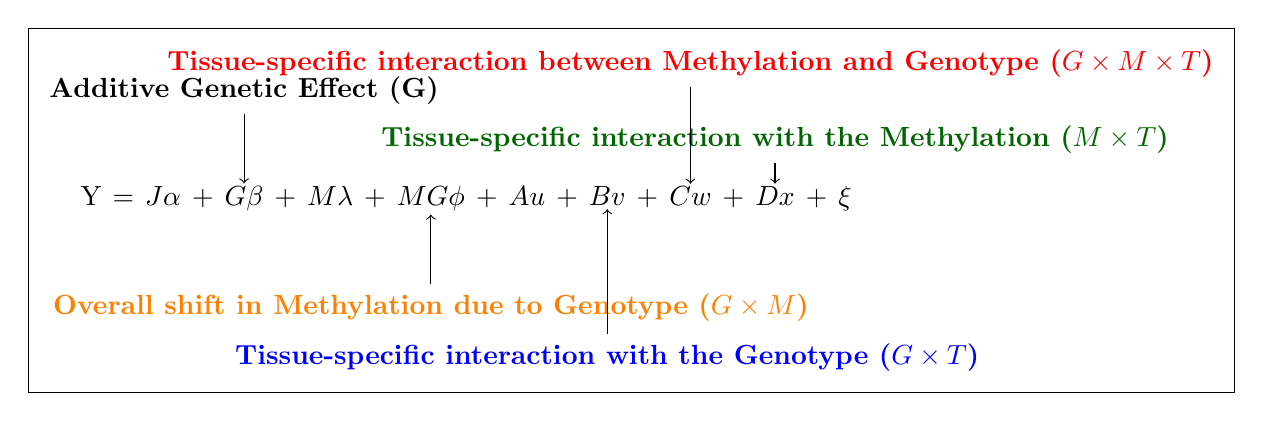
\begin{tikzpicture}[framed]
\matrix[name=M1, matrix of nodes, inner sep=1pt, column sep=2pt]{
      \node (Y) {Y}; & \node (equals) {=}; & \node (J) {$J\alpha$}; &+& \node (G) {$G\beta$}; &+& \node (M) {$M\lambda$}; &+& \node (MG) {$MG\phi$}; &+&  \node (A) {$Au$}; &+& \node (B) {$Bv$}; &+& \node (C) {$Cw$}; &+&  \node (D) {$Dx$}; &+& \node (F) {$\xi$};\\
    };
%    \node (Gene) [left=2.5em of Y] {\textbf{Gene Expression}};
    \node (VariableG) [above=2.5em of G] {\textbf{Additive Genetic Effect (G) }};
    \node (VariableB) [blue,below=4.5em of B] {\textbf{Tissue-specific interaction with the Genotype ($G \times T$)}};
    \node (VariableMG) [orange, below=2.5em of MG] {\textbf{Overall shift in Methylation due to Genotype ($G \times M$)}};
    \node (VariableC) [red, above=3.5em of C] {\textbf{Tissue-specific interaction between Methylation and Genotype ($G \times M \times T$)}};
    \node (VariableM) [black!60!green,above=0.75em of D] {\textbf{Tissue-specific interaction with the Methylation ($M \times T$)}};
%  \draw[->] (Gene) -- (Y);
    \draw[->] (VariableB) -- (B);
    \draw[->] (VariableG) -- (G);
    \draw[->] (VariableMG) -- (MG);
    \draw[->] (VariableC) -- (C);
    \draw[->] (VariableM) -- (D);
   
\end{tikzpicture}
\caption{Description of all the terms in our model}
\end{figure}

Parameters of interest are $\gamma$, $\delta$, $\beta$ and $\phi$; $\alpha$, $\lambda$, $\tau$, $\theta$ and $\epsilon$ are nuisance parameters. We test the null hypothesis that $H_0: \beta = \phi = \gamma =  \delta = 0$, i.e. the variant does not affect gene expression across any of the tissues. To do so, we compute the efficient scores for $\gamma$, $\delta$, $\beta$ and $\phi$ by projecting off components correlated with the nuisance parameters. 

%\[
%\large
%\Theta = \left\{ \gamma, \delta \right\} \quad and \quad \beta \quad and \quad \phi
%\]

%We define global null as --
%
%\begingroup
%\large
%\begin{center}
%$
%\boxed{
%H_0: \beta = \phi = \Theta = 0; \qquad H_A: \beta \neq 0; \phi \neq 0; \quad \Theta > 0
%}
%$
%\end{center}
%\endgroup
%
%The total variance under the global null is $\Sigma  = \epsilon I + \tau A A^{T} + \theta D D^T$.

From equation 1, the log-likelihood function of Y conditioned on the genotype is --

\begin{equation}
\ell \left( \Theta ;Y \right) =  - c - \frac{1}{2} \log \mid \Sigma \mid - \frac{1}{2} \left( Y  - J \alpha - G\beta - M\lambda - MG\phi \right )^T \Sigma ^{-1} \left( Y  - J \alpha - G\beta - M\lambda - MG\phi \right )
\end{equation}

where $\Theta$ represents the vector of all the variance components involved in $\Sigma$ and $c$ is a constant. Alternatively, under normality, we have

\[
Y \sim N( J\alpha + G\beta + M\lambda + MG\phi,\Sigma )
\]

The efficient scores evaluated under the null are given by --

\begingroup
\large
\begin{equation*}
U_\beta = \hat{Y}^T \hat{\Sigma}_n^{-1} \left( G - \bar{G} \right) \\
\end{equation*}
\endgroup

\begingroup
\large
\begin{equation*}
U_\phi = \hat{Y}^T \hat{\Sigma}_n^{-1} \left( MG - \overline{MG} \right) \\
\end{equation*}
\endgroup

\begingroup
\large
\begin{equation*}
U_\gamma = \frac{1}{2} \hat{Y}^T \hat{\Sigma}_n^{-1} BB^T \hat{\Sigma}_n^{-1} \hat{Y} \\
\end{equation*}
\endgroup

\begingroup
\large
\begin{equation*}
U_\delta = \frac{1}{2} \hat{Y}^T \hat{\Sigma}_n^{-1} CC^T \hat{\Sigma}_n^{-1} \hat{Y}\\
\end{equation*}
\endgroup

where $\hat{Y}$ are the residuals and $\hat{\Sigma} = \hat{\epsilon} I + \hat{\tau}ZZ^T + \hat{\theta}DD^T$.

We propose a weighted sum of the above components to arrive at our joint score test statistic, $U_\psi$. Since $U_\beta$ and $U_\phi$ are linear in $Y$ while $U_\gamma$ and $U_\delta$ are quadratic, we propose the following rule to combine them --	

\begingroup
\large
\begin{equation}
\begin{split}
U_\psi &\equiv  \left( \boldsymbol{a_\beta} U^2_\beta + \boldsymbol{a_\phi} U^2_\phi + \boldsymbol{a_\gamma} U_\gamma + \boldsymbol{a_\delta} U_\delta  \right) \\
 &\equiv \hat{Y}^T  \hat{\Sigma}_n^{-1} \left[ a_\beta \left(G - \bar{G}\right) \left(G - \bar{G}\right)^T  + a_\phi \left(MG - \overline{MG}\right) \left(MG - \overline{MG}\right)^T  + a_\gamma \frac{1}{2} B B^T + a_\delta \frac{1}{2} C C^T  \right]  \hat{\Sigma}_n^{-1} \hat{Y} \\
\end{split}
\end{equation}
\endgroup

where $a_\beta$, $a_\phi$, $a_\gamma$ and $a_\delta$ are scalar constants chosen to minimize the variance of $U_\psi$. Under the null, $U_\psi$ is distributed as a mixture of chi-square random variables. We use Satterthwaite method \cite{satterthwaite} to approximate the $p$~values from a scaled $\chi^2$ distribution by matching the first two moments as $U_\psi \sim \kappa \chi^2_{\nu}$ where $\kappa = \frac{2 Var(U_\psi)}{E[U_\psi]}$ and $\nu = \frac{2 E[U_\psi]^2}{Var(U_\psi)}$. 

Our joint score test will test for the effect of genotype on 1) an overall shift in the gene expression, 2) tissue-specific interaction ($G \times T$), 3) overall methylation ($G \times M$), and 4) tissue-specific methylation ($G \times M \times T$)

\section{Individual components of our joint score test statistic}

\subsection{Score test for the additive genetic effect on the gene expression under the global null}

\begin{center}
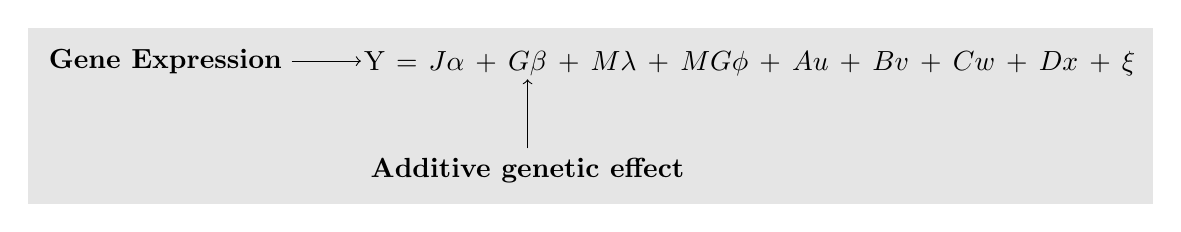
\begin{tikzpicture}[framed,show background rectangle,background rectangle/.style={fill=black!10}]]
\matrix[name=M1, matrix of nodes, inner sep=1pt, column sep=2pt]{
      \node (Y) {Y}; & \node (equals) {=}; & \node (J) {$J\alpha$}; &+& \node (G) {$G\beta$}; &+& \node (M) {$M\lambda$}; &+& \node (MG) {$MG\phi$}; &+&  \node (A) {$Au$}; &+& \node (B) {$Bv$}; &+& \node (C) {$Cw$}; &+&  \node (D) {$Dx$}; &+& \node (F) {$\xi$}; \\
       };
    \node (Gene) [left=2.5em of Y] {\textbf{Gene Expression}};
    \node (VariableG) [below=2.5em of G] {\textbf{Additive genetic effect}};
    \draw[->] (Gene) -- (Y);
    \draw[->] (VariableG) -- (G);
\end{tikzpicture}
\end{center}

The score test for the fixed effect $\beta$ takes the following form under the global null --

\begingroup
\large
\begin{equation}
U_\beta = \left( G - \bar{G} \right)^T\Sigma_n^{-1} \hat{Y} 
\end{equation}
\endgroup

where  $\left(G - \bar{G} \right)$ is a vector of mean-centered genotypes for all individuals and $\hat{Y} = \left( Y - J\hat{\alpha} - M\hat{\lambda}\right)$.  $U_\beta$ is a scalar quantity in a linear form and follows a $\chi^2_1$ distribution.

Squaring $U_\beta$ gives us the following quadratic form, which will be useful while aggregating all the score test statistics. 

\begingroup
\large
\begin{equation}
U^2_\beta = \hat{Y}^T \Sigma_n^{-1} \left(G - \bar{G}\right)\left(G - \bar{G}\right)^T \Sigma_n^{-1} \hat{Y} 
\end{equation}
\endgroup

\subsection{The effect of SNP on gene expression via differential methylation patterns under the global null ($G \times M$)}

\begin{center}
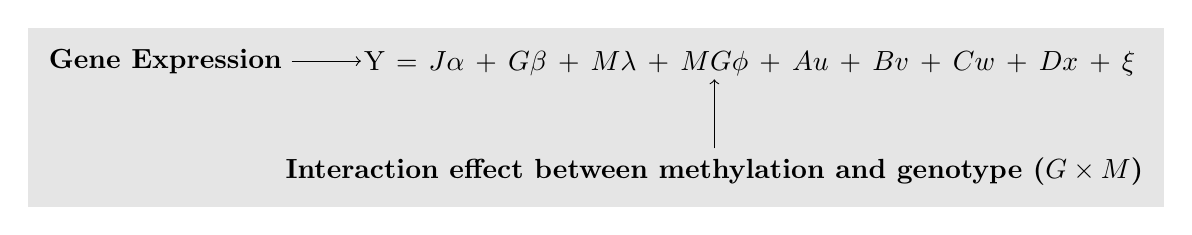
\begin{tikzpicture}[framed,show background rectangle,background rectangle/.style={fill=black!10}]]
\matrix[name=M1, matrix of nodes, inner sep=1pt, column sep=2pt]{
       \node (Y) {Y}; & \node (equals) {=}; & \node (J) {$J\alpha$}; &+& \node (G) {$G\beta$}; &+& \node (M) {$M\lambda$}; &+& \node (MG) {$MG\phi$}; &+&  \node (A) {$Au$}; &+& \node (B) {$Bv$}; &+& \node (C) {$Cw$}; &+&  \node (D) {$Dx$}; &+& \node (F) {$\xi$};\\
        };
    \node (Gene) [left=2.5em of Y] {\textbf{Gene Expression}};
    \node (VariableC) [below=2.5em of MG] {\textbf{Interaction effect between methylation and genotype ($G \times M$)}};
    \draw[->] (Gene) -- (Y);
    \draw[->] (VariableC) -- (MG);
\end{tikzpicture}
\end{center}

The score test for the interaction effect $\phi$ takes the following form under the global null --

\begingroup
\large
\begin{equation}
U_\phi = \left( MG - \overline{MG} \right)^T\Sigma_n^{-1} \hat{Y}
\end{equation}
\endgroup

where $\Sigma_n = diag\left(\Sigma, \cdots , \Sigma \right)$ is an $nt \times nt$ block diagonal matrix and $\hat{Y} = \left( Y - J\hat{\alpha} - M\hat{\lambda}\right)$. $U_\phi$ is a scalar quantity in a linear form and follows a $\chi^2_1$ distribution. Squaring $U_\phi$ gives us the following quadratic form, which will be useful while aggregating all the score test statistics. 

\begingroup
\large
\begin{equation}
U^2_\phi = \hat{Y}^T \Sigma_n^{-1} \left(MG - \overline{MG}\right)\left(MG - \overline{MG}\right)^T \Sigma_n^{-1} \hat{Y}
\end{equation}
\endgroup


\subsection {Variance-component score test for the tissue-specific effect due to genotype on the gene expression under the global null ($G \times T$)}

\begin{center}
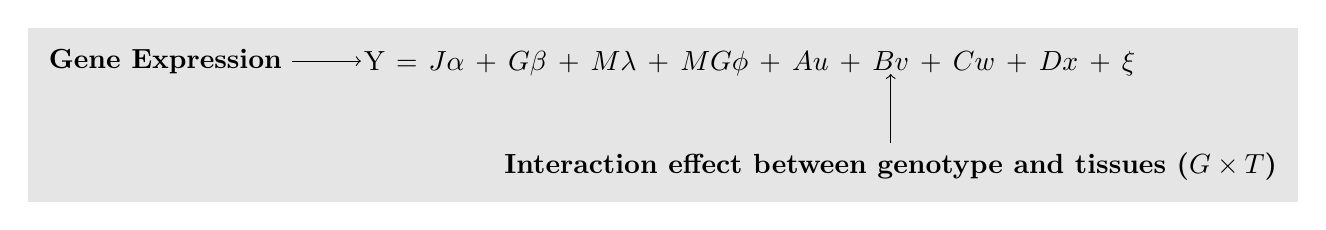
\begin{tikzpicture}[framed,show background rectangle,background rectangle/.style={fill=black!10}]]
\matrix[name=M1, matrix of nodes, inner sep=1pt, column sep=2pt]{
      \node (Y) {Y}; & \node (equals) {=}; & \node (J) {$J\alpha$}; &+& \node (G) {$G\beta$}; &+& \node (M) {$M\lambda$}; &+& \node (MG) {$MG\phi$}; &+&  \node (A) {$Au$}; &+& \node (B) {$Bv$}; &+& \node (C) {$Cw$}; &+&  \node (D) {$Dx$}; &+& \node (F) {$\xi$}; \\
       };
    \node (Gene) [left=2.5em of Y] {\textbf{Gene Expression}};
    \node (VariableB) [below=2.5em of B] {\textbf{Interaction effect between genotype and tissues ($G \times T$)}};
    \draw[->] (Gene) -- (Y);
    \draw[->] (VariableB) -- (B);
\end{tikzpicture}
\end{center}

The score for the variance component $\boldsymbol{\gamma}$ under the global null is --

\begingroup
\large
\begin{equation}
\frac{1}{2} \left\{ \hat{Y}^T \Sigma_n^{-1} BB^T \Sigma_n^{-1} \hat{Y} - Tr \left(\Sigma_n^{-1} BB^T\right)\right\}
\end{equation}
\endgroup

where $\Sigma_n = diag\left(\Sigma, \cdots , \Sigma \right)$ is an $nt \times nt$ block diagonal matrix and $\hat{Y} = \left( Y - J\hat{\alpha} - M\hat{\lambda}\right)$. As the \emph{trace} term does not depend on the data, we use the first term to construct the test statistic.

\begingroup
\large
\begin{equation}
U_\gamma = \frac{1}{2} \hat{Y}^T \Sigma_n^{-1} BB^T \Sigma_n^{-1} \hat{Y}
\end{equation}
\endgroup

$U_\gamma$ follows a mixture of chi-square distribution and the $p$~value is approximated using a scaled $\chi^2$ distribution (the Satterthwaite method) by matching the first two moments as $U_\gamma \sim \kappa \chi^2_{\nu}$ where $\kappa = \frac{2 Var(U_\gamma)}{E[U_\gamma]}$ and $\nu = \frac{2 E[U_\gamma]^2}{Var(U_\gamma)}$. 

\subsection{Latent effect (masking effect) of SNP on gene expression via tissue-specific methylation patterns ($G \times M \times T$)}

\begin{center}
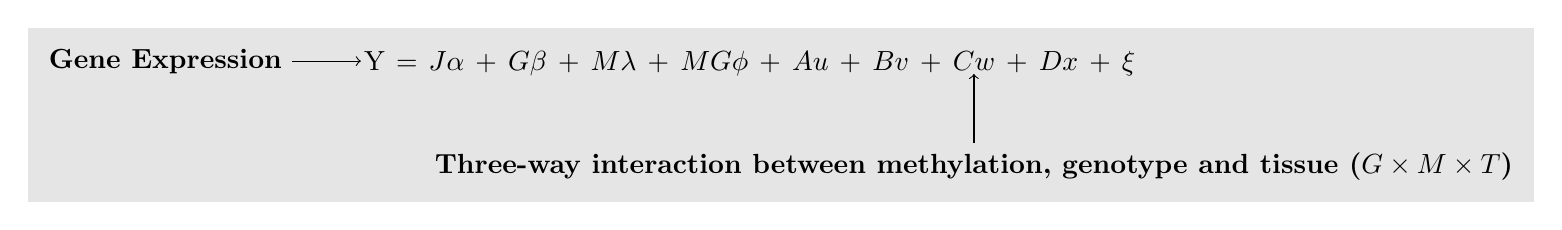
\begin{tikzpicture}[framed,show background rectangle,background rectangle/.style={fill=black!10}]]
\matrix[name=M1, matrix of nodes, inner sep=1pt, column sep=2pt]{
      \node (Y) {Y}; & \node (equals) {=}; & \node (J) {$J\alpha$}; &+& \node (G) {$G\beta$}; &+& \node (M) {$M\lambda$}; &+& \node (MG) {$MG\phi$}; &+&  \node (A) {$Au$}; &+& \node (B) {$Bv$}; &+& \node (C) {$Cw$}; &+&  \node (D) {$Dx$}; &+& \node (F) {$\xi$}; \\
       };
    \node (Gene) [left=2.5em of Y] {\textbf{Gene Expression}};
    \node (VariableC) [below=2.5em of C] {\textbf{Three-way interaction between methylation, genotype and tissue ($G \times M \times T$)}};
    \draw[->] (Gene) -- (Y);
    \draw[->] (VariableC) -- (C);
\end{tikzpicture}
\end{center}

The score for the variance component $\boldsymbol{\delta}$ under the global null is --

\begingroup
\large
\begin{equation}
\frac{1}{2} \left\{\hat{Y}^T \Sigma_n^{-1} CC^T \Sigma_n^{-1} \hat{Y} - Tr \left(\Sigma_n^{-1} CC^T\right)\right\}
\end{equation}
\endgroup

where $\Sigma_n = diag\left(\Sigma, \cdots , \Sigma \right)$ is an $nt \times nt$ block diagonal matrix and $\hat{Y} = \left( Y - J\hat{\alpha} - M\hat{\lambda}\right)$. As the \emph{trace} term does not depend on the data, we use the first term to construct the test statistic.

\begingroup
\large
\begin{equation}
U_\delta = \frac{1}{2}\hat{Y}^T \Sigma_n^{-1} CC^T \Sigma_n^{-1} \hat{Y}
\end{equation}
\endgroup

$U_\delta$ follows a mixture of chi-square distribution, the $p$~value can be approximated using a scaled $\chi^2$ distribution by matching the first two moments as $U_\delta \sim \kappa \chi^2_{\nu}$ where $\kappa = \frac{2 Var(U_\delta)}{E[U_\delta]}$ and $\nu = \frac{2 E[U_\delta]^2}{Var(U_\delta)}$. 

\section{Simulations}

General descriptions of the simulations --

\begin{itemize}
\item For each tissue, we model the potential genetic association between \underline{a target SNP} and the expression levels of \underline{a target gene} at a \underline{single locus}. 
\item \underline{Methylation data} is generated independently from a multivariate normal distribution with a positive semi-definite variance-covariance matrix.
\item We have generated one gene and one SNP at a time with the genotypes at each SNP in each individual simulated assuming Hardy-Weinberg equilibrium with varying minor allele frequencies (MAF). 
%\item Tissue-specific interaction effect due to genotype was created by varying $\gamma$, tissue-specific interaction effect due to methylation was created by varying $\phi$ and tissue-specific interaction with the genotype and methylation was created by varying $\delta$. 
\item All the simulations are performed on 5 tissues, 100 observations in each tissue, and genotypes follow common variant frequency (MAF = 0.30).
\item For all null simulations, $\theta = \tau = \epsilon = 1$. 
\item The proportion of variance explained (PVE) by $\gamma$ and $\delta$ are defined as:
\[
\large
PVE_{\gamma} \equiv \left(\frac{\gamma}{\theta + \tau + \epsilon + \gamma + \delta }\right)  \qquad PVE_{\delta} \equiv \left(\frac{\delta}{\theta + \tau + \epsilon + \gamma + \delta}\right) 
\]
\end{itemize}

\subsection{Evaluating the joint score test}

Each simulated dataset was comprised of data from a single locus and a single gene, whose expression is measured across 5 tissues in 100 observations. For a given gene-SNP pair, the genotypes at each SNP in all the individuals were simulated as Binomial(2,0.3), i.e. a minor allele frequency 30\% and assuming Hardy-Weinberg equilibrium. Methylation data for 5 tissues was generated from a multivariate normal distribution with zero mean and an identity matrix as a covariance matrix. The gene expression data are generated prospectively, i.e., first genotypes are generated, followed by gene expression according to the following equation --
\begingroup
\large
\begin{equation}
y_{it} = \alpha_t + \beta_i g_i + \lambda_i m_{it} + \phi_i m_{it} g_i + a_i + b_t g_i + c_t m_{it} g_i + d_t m_{it} + \xi_{it} \qquad \xi  \overset{i.i.d.} \sim N \left( 0, \epsilon \right)
\end{equation}
\endgroup

where $y_{it}$ is a vector of gene expression data, $\alpha_t$ is the tissue-specific intercept, $\beta$ describes the main additive genotypic effect, $\lambda$ describes the overall effect due to methylation, $\phi$ describes the interaction effect between the overall methylation and genotype,  $g$ is the value of a bi-allelic genotype such that $g \in \left(0,1,2\right)$ represents the number of copies of the minor allele. The random effect $b_t$ represents tissue-specific effect of the genotype, $c_t$ represents tissue-specific interaction effect between methylation and genotype, $d_t$ represents tissue-specific methylation effect, and $a_i$ is a subject-specific random intercept. We assume that the random effects are independent and that $a_i \sim N_t \left(0, \tau \right)$, $b_t \sim N_t \left(0, \gamma \right)$, $c_t \sim N_t \left(0,\delta\right)$ and $d_t \sim N_t \left(0,\theta\right)$. 

We use 1,000 data replicates to evaluate type I error and power calculations. Simulations were performed by varying $\beta$, the proportion of variance explained by the random effect describing the interaction between genotype and tissue, $PVE_{\gamma} \equiv \left(\frac{ \gamma}{\theta + \tau + \epsilon + \gamma + \delta }\right)$, and the proportion of variance explained by the random effect describing the interaction between genotype, methylation and tissue, $PVE_{\delta} \equiv \left(\frac{ \delta}{\theta + \tau + \epsilon + \gamma + \delta}\right)$. A linear mixed effects model was fit using the package \emph{lme4} \cite{lme4} in the statistical environment R (R Core Team) \cite{R}.

\begin{longtable}{lllllllll}
\hline
$\beta$ & $\phi$  & $PVE_\delta (\%)$  & $PVE_\gamma (\%)$  &  $U_{\beta|H_0}$ & $U_{\phi|H_0}$ & $U_{\gamma|H_0}$ & $U_{\delta|H_0}$ & $U_{\psi|H_0}$ \\ \hline
\endfirsthead
$\beta$ & $\phi$  & $PVE_\delta (\%)$  & $PVE_\gamma (\%)$  &  $U_{\beta|H_0}$ & $U_{\phi|H_0}$ & $U_{\gamma|H_0}$ & $U_{\delta|H_0}$ & $U_{\psi|H_0}$ \\ \hline
\endhead
\multicolumn{9}{r}{{Continued\ldots}} \
\endfoot
\hline
\endlastfoot
NO & NO & 0 & 0 & 0.058 & 0.045 & 0.061 & 0.053 & 0.06 \\
NO & NO & 0 & 5 & 0.071 & 0.055 & 0.278 & 0.052 & 0.161 \\
NO & NO & 0 & 8 & 0.092 & 0.064 & 0.602 & 0.062 & 0.427 \\
NO & NO & 5 & 0 & 0.053 & 0.151 & 0.047 & 0.28 & 0.173 \\
NO & NO & 5 & 5 & 0.079 & 0.153 & 0.294 & 0.288 & 0.325 \\
NO & NO & 5 & 8 & 0.107 & 0.143 & 0.641 & 0.274 & 0.571 \\
NO & NO & 8 & 0 & 0.055 & 0.251 & 0.072 & 0.549 & 0.383 \\
NO & NO & 8 & 5 & 0.081 & 0.255 & 0.312 & 0.622 & 0.585 \\
NO & NO & 8 & 8 & 0.107 & 0.263 & 0.645 & 0.604 & 0.734 \\	\hdashline
NO & YES & 0 & 0 & 0.058 & 0.883 & 0.039 & 0.674 & 0.171 \\
NO & YES & 0 & 5 & 0.08 & 0.884 & 0.28 & 0.696 & 0.385 \\
NO & YES & 0 & 8 & 0.101 & 0.888 & 0.629 & 0.674 & 0.616 \\
NO & YES & 5 & 0 & 0.047 & 0.825 & 0.061 & 0.772 & 0.381 \\
NO & YES & 5 & 5 & 0.065 & 0.844 & 0.314 & 0.751 & 0.525 \\
NO & YES & 5 & 8 & 0.102 & 0.834 & 0.611 & 0.747 & 0.725 \\
NO & YES & 8 & 0 & 0.071 & 0.762 & 0.072 & 0.83 & 0.573 \\
NO & YES & 8 & 5 & 0.084 & 0.76 & 0.309 & 0.837 & 0.677 \\
NO & YES & 8 & 8 & 0.099 & 0.719 & 0.579 & 0.848 & 0.826 \\ \hline
YES & NO & 0 & 0 & 0.287 & 0.05 & 0.054 & 0.045 & 0.208 \\
YES & NO & 0 & 5 & 0.308 & 0.058 & 0.295 & 0.055 & 0.357 \\
YES & NO & 0 & 8 & 0.322 & 0.059 & 0.648 & 0.056 & 0.588 \\
YES & NO & 5 & 0 & 0.303 & 0.127 & 0.053 & 0.275 & 0.355 \\
YES & NO & 5 & 5 & 0.301 & 0.147 & 0.291 & 0.253 & 0.484 \\
YES & NO & 5 & 8 & 0.356 & 0.116 & 0.642 & 0.249 & 0.689 \\
YES & NO & 8 & 0 & 0.325 & 0.279 & 0.064 & 0.566 & 0.585 \\
YES & NO & 8 & 5 & 0.323 & 0.268 & 0.306 & 0.584 & 0.68 \\
YES & NO & 8 & 8 & 0.329 & 0.284 & 0.631 & 0.606 & 0.823 \\	\hdashline
YES & YES & 0 & 0 & 0.322 & 0.916 & 0.062 & 0.693 & 0.421 \\
YES & YES & 0 & 5 & 0.327 & 0.88 & 0.308 & 0.669 & 0.552 \\
YES & YES & 0 & 8 & 0.341 & 0.89 & 0.637 & 0.691 & 0.74 \\
YES & YES & 5 & 0 & 0.318 & 0.81 & 0.084 & 0.742 & 0.57 \\
YES & YES & 5 & 5 & 0.305 & 0.809 & 0.294 & 0.734 & 0.666 \\
YES & YES & 5 & 8 & 0.349 & 0.802 & 0.589 & 0.757 & 0.809 \\
YES & YES & 8 & 0 & 0.288 & 0.761 & 0.076 & 0.832 & 0.705 \\
YES & YES & 8 & 5 & 0.32 & 0.767 & 0.333 & 0.84 & 0.816 \\
YES & YES & 8 & 8 & 0.351 & 0.737 & 0.623 & 0.817 & 0.869 \\
\hline \hline
\caption{Table comparing the statistical power of the joint score test statistic, $U_\psi$ and the contributions from its main components, $U_\beta$, $U_\gamma$ and $U_\delta$, all under the global null. These data were generated from 1,000 simulations run on 100 individuals and five tissues with genotypes generated at a common variant allele frequency (MAF = 0.3). }
\end{longtable}

\subsection{Comparing tissue-by-tissue approach with our joint score test statistic}

A tissue-by-tissue (TBT) analysis fits the following model \textbf{Gene $\sim$ CpG + Geno + Geno:CpG} in individual tissues. For tissue $t$ and SNP $j$, the gene expression is modeled as a function of the genotype and methylation data:

\begingroup
\large
\begin{equation}
Y_{t} =  \alpha_j m_{t} + \beta_t g_j + \delta_t g_j m_{t} + \epsilon_t
\end{equation}
\endgroup

where $Y_t$ is the gene expression $g$ of individuals in tissue $t$, $g_j$ is the genotype data on SNP $j$, $m_t$ is methylation information in tissue $t$. Minimum $p$~value from the TBT analysis across all the tissues is computed for power calculations.

\begin{longtable}{llllll}
\hline
$\beta$ & $\phi$ & $PVE_\delta  (\%)$ & $PVE_\gamma  (\%)$ & TBT & $U_\psi$ \\ \hline
\endfirsthead
$\beta$ & $\phi$ & $PVE_\delta  (\%)$ & $PVE_\gamma  (\%)$ & TBT & $U_\psi$ \\ \hline
\endhead
\multicolumn{6}{r}{{Continued\ldots}} \
\endfoot
\hline
\endlastfoot
NO & NO & 0 & 0 & 0.053 & 0.056 \\
NO & NO & 0 & 7 & 0.097 & 0.171 \\
NO & NO & 0 & 10 & 0.222 & 0.425 \\
NO & NO & 7 & 0 & 0.18 & 0.195 \\
NO & NO & 7 & 7 & 0.202 & 0.303 \\
NO & NO & 7 & 10 & 0.368 & 0.55 \\
NO & NO & 10 & 0 & 0.426 & 0.429 \\
NO & NO & 10 & 7 & 0.453 & 0.523 \\
NO & NO & 10 & 10 & 0.554 & 0.719 \\ \hdashline
NO & YES & 0 & 0 & 0.325 & 0.179 \\
NO & YES & 0 & 7 & 0.396 & 0.361 \\
NO & YES & 0 & 10 & 0.522 & 0.618 \\
NO & YES & 7 & 0 & 0.519 & 0.355 \\
NO & YES & 7 & 7 & 0.584 & 0.519 \\
NO & YES & 7 & 10 & 0.66 & 0.706 \\
NO & YES & 10 & 0 & 0.669 & 0.588 \\
NO & YES & 10 & 7 & 0.706 & 0.697 \\
NO & YES & 10 & 10 & 0.779 & 0.805 \\ \hline
YES & NO & 0 & 0 & 0.143 & 0.235 \\
YES & NO & 0 & 7 & 0.248 & 0.365 \\
YES & NO & 0 & 10 & 0.392 & 0.586 \\
YES & NO & 7 & 0 & 0.288 & 0.395 \\
YES & NO & 7 & 7 & 0.393 & 0.526 \\
YES & NO & 7 & 10 & 0.512 & 0.698 \\
YES & NO & 10 & 0 & 0.514 & 0.566 \\
YES & NO & 10 & 7 & 0.589 & 0.696 \\
YES & NO & 10 & 10 & 0.683 & 0.812 \\ \hdashline
YES & YES & 0 & 0 & 0.48 & 0.4 \\
YES & YES & 0 & 7 & 0.549 & 0.541 \\
YES & YES & 0 & 10 & 0.678 & 0.747 \\
YES & YES & 7 & 0 & 0.641 & 0.588 \\
YES & YES & 7 & 7 & 0.686 & 0.683 \\
YES & YES & 7 & 10 & 0.754 & 0.83 \\
YES & YES & 10 & 0 & 0.772 & 0.721 \\
YES & YES & 10 & 7 & 0.765 & 0.789 \\
YES & YES & 10 & 10 & 0.847 & 0.898 \\
\hline \hline
\caption{Table comparing the statistical power of the joint score test statistic, $U_\psi$ and TBT approach. This data were generated from 1,000 simulations run on 100 individuals and five tissues with genotypes generated at a common variant allele frequency (MAF = 0.3).}
\end{longtable}

Our joint model clearly outperforms TBT analysis in terms of statistical power.

\subsection{Leveraging methylation data to improve eQTL discovery}

We proposed a method, JAGUAR \cite{jaguar}, which investigated the presence of two types of genetic effects: 1) an overall shift in gene expression due to genotype across all tissues, and 2) tissue-specific effects of genotypes on gene expression using the following linear model --

\begin{equation}
Y = J\alpha + G\beta + Au + Bv + \xi \qquad Y \sim N\left(J\alpha + G\beta, \sigma\right)
\end{equation}
where $Y$ is a $nt$-dimensional vector of expression levels in $t$ tissues and $n$ individuals, $\alpha$ is a vector of tissue-specific intercepts, $G$ is a $nt$-dimensional vector of genotypes, $\beta$ is a fixed effect of genotype across tissue, $u \sim N\left(0, \tau AA^T \right)$ is a vector of subject-specific random effect, $v \sim N\left(0,\gamma BB^T \right)$ is a vector of tissue-specific random effects, and $\xi \sim N\left(0, \epsilon I_{nt} \right)$. The matrices $J$, $A$ and $B$ are design matrices with $B$ being a function of genotype. $J$ is $nt \times t$ dimensional matrix denoting the design matrix for the tissue-specific intercepts. $A$ is $nt \times nt$ design matrix for the subject-specific intercepts. $B$ is a $nt \times t$ design matrix of stacked genotypes. The parameters of interest are $\beta$ and $\gamma$; $\alpha$, $\tau$ and $\epsilon$ are nuisance parameters.

We ask if including the terms associated with the methylation data to the above equation may lead to any substantial power loss. In order to do this, we keep all the variance components and fixed effects associated with methylation in equation 1 at zero (i.e. $\lambda$ = $\phi$ = $\delta$ = $\theta$ = 0). Statistical power from the joint analysis of only genotype and tissue-specific interaction using JAGUAR \cite{jaguar_cran} made available at Comprehensive R Archive Network (CRAN) repository \url{https://cran.r-project.org/web/packages/JAGUAR/index.html} was compared with our new method. As seen in figure 4, the loss of statistical power is not substantial. 
\begin{center}
\begin{figure}[!ht]
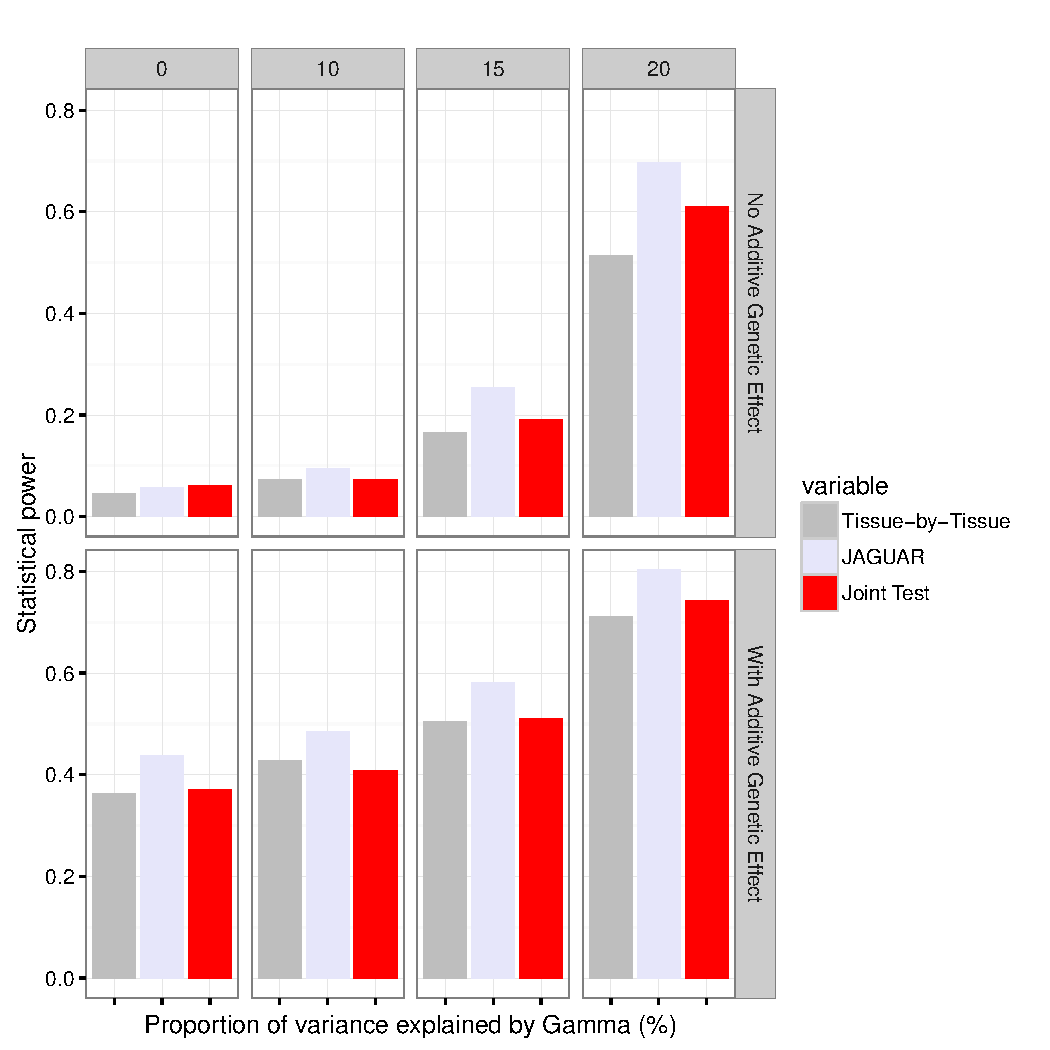
\includegraphics[width=\textwidth]{JT_JAG_TBT.pdf}
\caption{Comparing TBT, JAGUAR and the joint score test approaches.  In the absence of methylation data, statistical power from the joint analysis of genotype and tissue-specific interaction using JAGUAR is marginally better than our joint score test. A tissue-by-tissue method is also used for comparison. These data were generated from 1,000 simulations run on 100 individuals and five tissues with genotypes generated at a common variant allele frequency (MAF = 0.3).}
\end{figure}
\end{center}
Similarly, figure 5 illustrates that in cases where methylation data effects gene expression via genetic variation, our model outperforms JAGUAR and a tissue-by-tissue approach.
\begin{center}
\begin{figure}[!ht]
%\resizebox{.8\textwidth}{!}{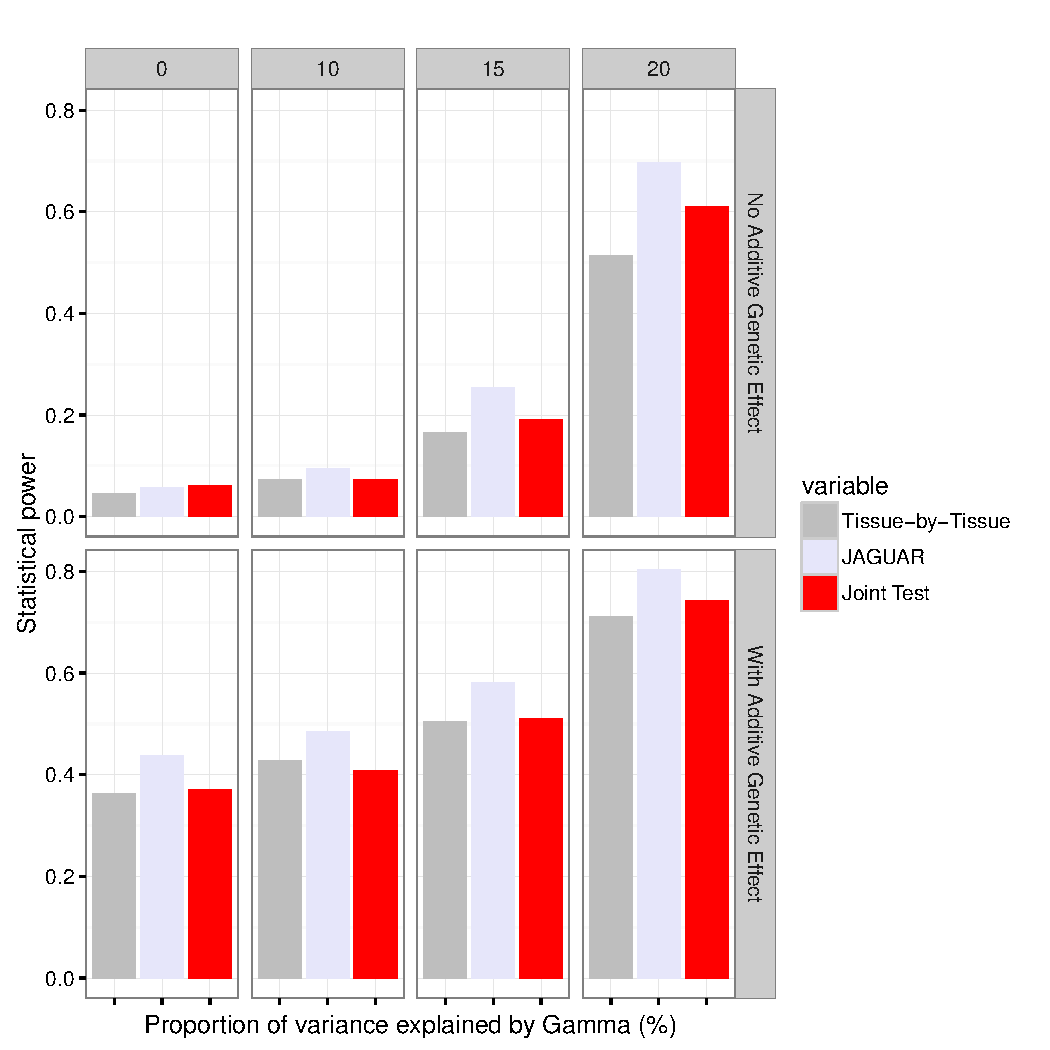
\includegraphics{JT_JAG_TBT.pdf}}
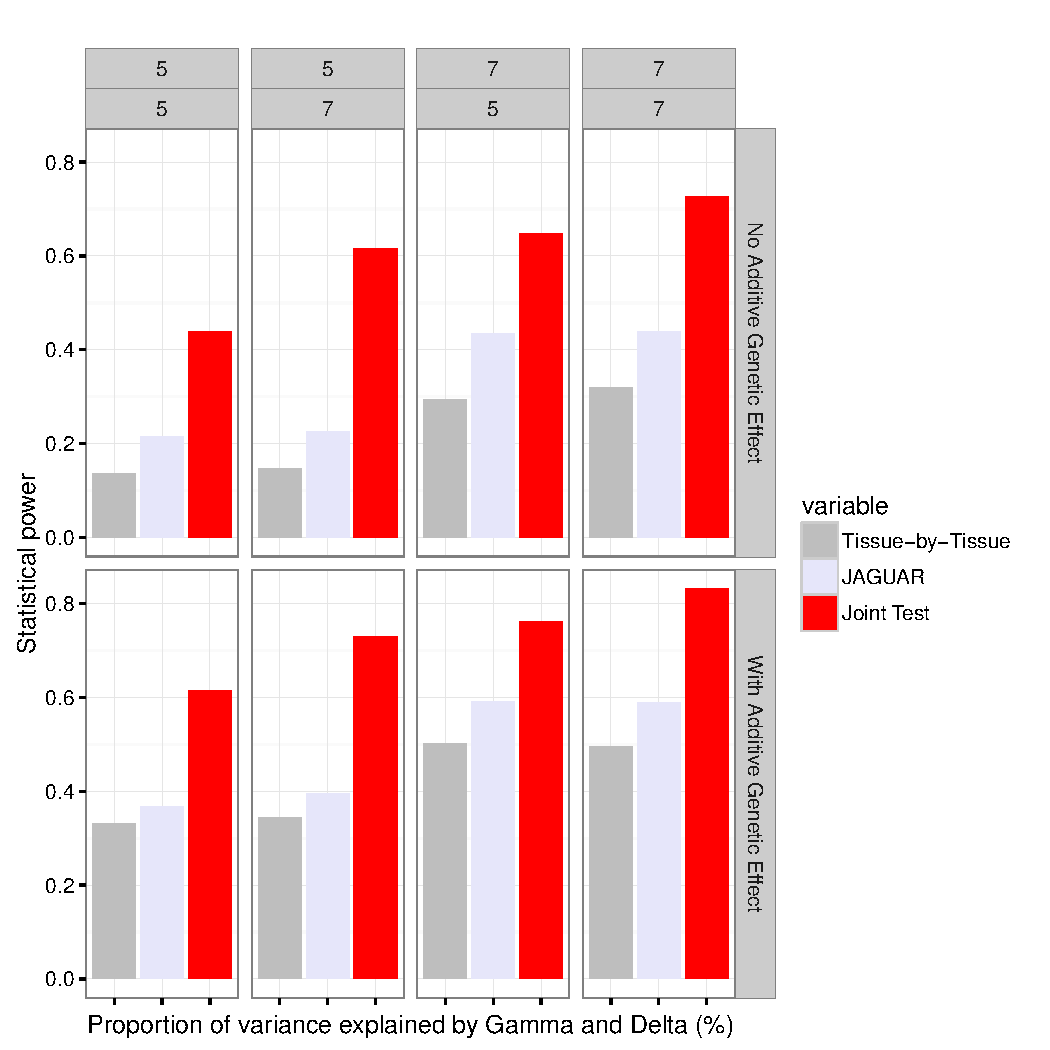
\includegraphics[width=\textwidth]{JT_JAG_TBT_Jan27.pdf}
\caption{Comparing TBT, JAGUAR and the joint score test approaches. In the presence of DNA methylation effect, our method out performs JAGUAR and tissue-by-tissue analyses. The top two rows in the figure indicate $PVE_\gamma$ and $PVE_\delta$. These data were generated from 1,000 simulations run on 100 individuals and five tissues with genotypes generated at a common variant allele frequency (MAF = 0.3).}
\end{figure}
\end{center}

\subsection{Comparing the joint score test with $G \times M \times T$ interaction effect using a variance-component score test}

Given that --

\begin{center}
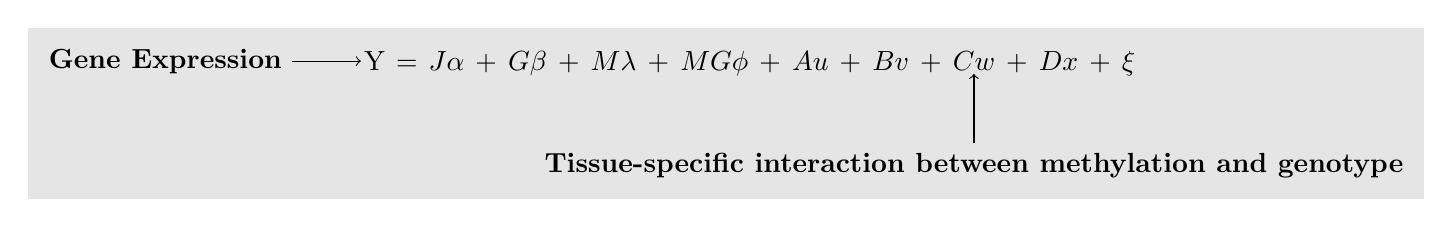
\begin{tikzpicture}[framed,show background rectangle,background rectangle/.style={fill=black!10}]]
\matrix[name=M1, matrix of nodes, inner sep=1pt, column sep=2pt]{
       \node (Y) {Y}; & \node (equals) {=}; & \node (J) {$J\alpha$}; &+& \node (G) {$G\beta$}; &+& \node (M) {$M\lambda$}; &+& \node (MG) {$MG\phi$}; &+&  \node (A) {$Au$}; &+& \node (B) {$Bv$}; &+& \node (C) {$Cw$}; &+&  \node (D) {$Dx$}; &+& \node (F) {$\xi$};\\
        };
    \node (Gene) [left=2.5em of Y] {\textbf{Gene Expression}};
    \node (VariableC) [below=2.5em of C] {\textbf{Tissue-specific interaction between methylation and genotype}};
    \draw[->] (Gene) -- (Y);
    \draw[->] (VariableC) -- (C);
\end{tikzpicture}
\end{center}

where $Y$ is a $nt$-dimensional vector of expression levels in $t$ tissues and $n$ individuals, $\alpha$ is a vector of tissue-specific intercepts, $G$ is a $nt$-dimensional vector of genotypes, $\beta$ is a fixed effect of genotype across tissue, $\lambda$ is an overall methylation-specific fixed effect, $\phi$ is genotype $\times$ methylation interaction effect (fixed effect), $u \sim N\left(0, \tau AA^T \right)$ is a vector of subject-specific random effect, $v \sim N\left(0,\gamma BB^T \right)$ is a vector of tissue-specific random effects, $w \sim N\left(0,\delta CC^T \right)$  is a vector of tissue-specific random effects that describe the interaction effect between genotype and methylation is a vector of random effects describing the interaction between genotype, methylation and tissue, $x \sim N\left(0,\theta DD^T \right)$ is a vector of tissue-specific random effects describing methylation effects and $\xi \sim N\left(0, \epsilon I_{nt} \right)$. The matrices $J$, $A$, $B$, $C$, and $D$ are design matrices with $B$ being a function of genotype, $C$ is a function of both genotype and methylation data and finally, $D$ is a function of just the methylation data. $J$ is $nt \times t$ dimensional matrix denoting the design matrix for the tissue-specific intercepts. $A$ is $nt \times nt$ design matrix for the subject-specific intercepts. $B$ is a $nt \times t$ design matrix of stacked genotypes. $C$ is a $nt \times t$ design matrix of stacked (product of) tissue-specific methylation and genotype data. $D$ is $nt \times t$ design matrices of stacked tissue-specific methylation data. 

Parameter of interest is $\delta$; $\alpha$, $\beta$, $\lambda$, $\phi$, $\tau$, $\gamma$, $\theta$ and $\epsilon$ are nuisance parameters. We test the null hypothesis that $H_0: \delta = 0$, i.e. there is no effect of genotype on tissue-specific methylation expression pattern. To do so, we compute the efficient scores for $\delta$ by projecting off components correlated with the nuisance parameters. 

The log-likelihood function of Y conditioned on the genotype is --

\begin{equation}
\ell \left( \Theta ;Y \right) =  - c - \frac{1}{2} \log \mid \Sigma \mid - \frac{1}{2} \left( Y  - J \alpha - G\beta - M\lambda - MG\phi \right )^T \Sigma ^{-1} \left( Y  - J \alpha - G\beta - M\lambda - MG\phi \right )
\end{equation}

where $\Theta$ represents the vector of all the variance components involved in $\Sigma$ and $c$ is a constant. Alternatively, under normality, we have

\[
Y \sim N( J\alpha + G\beta + M\lambda + MG\phi,\Sigma )
\]

The efficient scores evaluated under the null are given by --

\begingroup
\large
\begin{equation}
\frac{1}{2} \left\{\hat{Y}^T \Sigma_n^{-1} CC^T \Sigma_n^{-1} \hat{Y} - Tr \left(\Sigma_n^{-1} CC^T\right)\right\}
\end{equation}
\endgroup

In order to test the effect of interaction between SNP and tissue-specific methylation data on gene expression data, we test the following constrained hypothesis --

\begingroup
\large
\begin{center}
$
H_0: \delta = 0 \quad \and H_A: \delta > 0
$
\end{center}
\endgroup

As the null-hypothesis is now on the boundary of the parameter space, classical inferences using likelihood ratio is no longer applicable. 

\begin{table}[H]
\begin{center}
\begin{tabular}{| p{5cm} | c | c | c |}
\hline
& Hypotheses tested & Parameters of interest & Nuisance parameters \\ \hline
$G\times M \times T$ & $H_0: \delta = 0 \quad H_A: \delta > 0$ & $\delta$ & $\alpha$, $\lambda$, $\beta$, $\phi$, $\gamma$, $\tau$ and $\epsilon$ \\ \hline
Joint score test & $H_0: \beta = \Theta = 0 \quad H_A: \Theta > 0; \beta \neq 0 $ & $\beta$, $\gamma$, $\delta$ and $\phi$ & $\theta$, $\alpha$, $\lambda$, $\tau$ and $\epsilon$ \\ \hline
\end{tabular}
\end{center}
\caption{Hypothesis description}
\end{table}

A score test statistic can be constructed to test for this effect by projecting off all the components associated with the nuisance parameters.

\begingroup
\large
\[
\ddot{U}_\delta = \hat{Y}^T \hat{\Sigma}^{-1} CC^T \hat{\Sigma}^{-1} \hat{Y}
\]
\endgroup

where $\hat{\Sigma} = \hat{\tau}AA^T + \hat{\gamma}BB^T + \hat{\theta}DD^T  + \hat{\epsilon}I_n$. Under the null, $\ddot{U}_\delta$ is distributed as a mixture of chi-square random variables. We use Satterthwaite method to approximate the $p$~values from a scaled $\chi^2$ distribution by matching the first two moments as $\ddot{U}_\delta \sim \kappa \chi^2_{\nu}$ where $\kappa = \frac{2 Var(\ddot{U}_\delta)}{E[\ddot{U}_\delta]}$ and $\nu = \frac{2 E[\ddot{U}_\delta]^2}{Var(\ddot{U}_\delta)}$.

As a comparison, we have also conducted a likelihood ratio test (RLRT) analysis \cite{rlrsim}, which has the same asymptotic distribution as that of a score test. 

\begin{longtable}{lclclclclclc|c|}
\hline
$\beta$ & $\phi$  & $PVE_\delta (\%)$  & $PVE_\gamma (\%)$  &  $\ddot{U}_\delta$ & RLRT & $U_\psi$  \\ \hline
\endfirsthead
$\beta$ & $\phi$ & $PVE_\delta (\%)$  & $PVE_\gamma (\%)$  &  $\ddot{U}_\delta$ & RLRT & $U_\psi$  \\ \hline
\endhead
\multicolumn{7}{c}{{Continued\ldots}} \
\endfoot
\hline
\endlastfoot
NO & NO & 0 & 0 & 0.061 & 0.053 & 0.058 \\
NO & NO & 0 & 5 & 0.056 & 0.049 & 0.173 \\
NO & NO & 5 & 8 & 0.051 & 0.037 & 0.411 \\
NO & NO & 5 & 0 & 0.255 & 0.236 & 0.153 \\
NO & NO & 5 & 5 & 0.246 & 0.225 & 0.303 \\
NO & NO & 8 & 8 & 0.241 & 0.219 & 0.551 \\
NO & NO & 8 & 0 & 0.534 & 0.519 & 0.395 \\
NO & NO & 8 & 5 & 0.523 & 0.499 & 0.534 \\
NO & NO & 8 & 8 & 0.53 & 0.51 & 0.726 \\ \hdashline
NO & YES & 0 & 0 & 0.053 & 0.042 & 0.052 \\
NO & YES & 0 & 5 & 0.053 & 0.048 & 0.156 \\
NO & YES & 0 & 8 & 0.058 & 0.05 & 0.442 \\
NO & YES & 5 & 0 & 0.283 & 0.26 & 0.175 \\
NO & YES & 5 & 5 & 0.236 & 0.223 & 0.306 \\
NO & YES & 5 & 8 & 0.261 & 0.253 & 0.588 \\
NO & YES & 8 & 0 & 0.537 & 0.534 & 0.437 \\
NO & YES & 8 & 5 & 0.532 & 0.516 & 0.531 \\
NO & YES & 8 & 8 & 0.574 & 0.549 & 0.749 \\ \hline
YES & NO & 0 & 0 & 0.064 & 0.059 & 0.426 \\
YES & NO & 0 & 5 & 0.058 & 0.052 & 0.583 \\
YES & NO & 0 & 8 & 0.059 & 0.045 & 0.769 \\
YES & NO & 5 & 0 & 0.218 & 0.211 & 0.556 \\
YES & NO & 5 & 5 & 0.255 & 0.24 & 0.685 \\
YES & NO & 5 & 8 & 0.249 & 0.218 & 0.814 \\
YES & NO & 8 & 0 & 0.55 & 0.525 & 0.721 \\
YES & NO & 8 & 5 & 0.542 & 0.528 & 0.795 \\
YES & NO & 8 & 8 & 0.556 & 0.541 & 0.885 \\ \hdashline
YES & YES & 0 & 0 & 0.056 & 0.05 & 0.433 \\
YES & YES & 0 & 5 & 0.044 & 0.037 & 0.583 \\
YES & YES & 0 & 8 & 0.057 & 0.047 & 0.743 \\
YES & YES & 5 & 0 & 0.283 & 0.275 & 0.573 \\
YES & YES & 5 & 5 & 0.27 & 0.249 & 0.721 \\
YES & YES & 8 & 8 & 0.225 & 0.206 & 0.797 \\
YES & YES & 8 & 0 & 0.547 & 0.53 & 0.718 \\
YES & YES & 8 & 5 & 0.516 & 0.507 & 0.805 \\
YES & YES & 0 & 8 & 0.542 & 0.529 & 0.875 \\
\hline\hline
\caption{Table comparing the statistical power of the joint score test statistic, $U_\psi$, RLRT and $\ddot{U}_{\delta}$. This data were generated from 1,000 simulations run on 100 individuals and five tissues with genotypes generated at a common variant allele frequency (MAF = 0.3). }
\end{longtable}

\section{Analysis of Gibbs \emph{et al} adult normal human brain data}

\subsection{Data description}
Fresh frozen tissue samples of the cerebellum (CRBLM), frontal cortex (FCTX), caudal pons (PONS) and temporal cortex (TCTX) were obtained from 150 neuropathologically normal samples \cite{gibbs}. Genotyping was performed using Infinium HumanHap550 beadchips (Illumina) to assay genotypes for 561,466 SNPs, from the cerebellum tissue samples. CpG methylation status was determined using HumanMethylation27 BeadChips (Illumina), which measure methylation at 27,578 CpG dinucleotides at 14,495 genes. Profiling of 22,184 mRNA transcripts was performed using HumanRef-8 Expression BeadChips (Illumina) The datasets are publicly available (GEO Accession Number: \textbf{GSE15745}; dbGAP Study Accession: \textbf{phs000249.v1.p1}). 

\begin{table}[H]
\begin{center}
\resizebox{\linewidth}{!}{
\begin{tabular}{| c | c | c | p{3cm} | c |}
\hline
Accession ID & Repository & Data type & Platform & Number of probes \\ \hline \hline
GSE15745 & GEO & Gene expression data & Illumina humanRef-8 v2.0 expression beadchip & 22,184 \\ \hline
GSE15745 & GEO & Methylation data & Illumina HumanMethylation27 BeadChip & 27,578 \\ \hline
phs000249.v1.p1 & dbGaP & Genotype data & HumanHap550v3.0 7& 561,466 \\ \hline
\hline\hline
\end{tabular}
}
\label{table:design}
\end{center}
\caption{\emph{A description of brain data}}
\end{table}

\subsection{Data analysis design}
We performed data analyses that focused on \underline{\emph{cis} candidate regions}. 
\begin{itemize}
\item The proximity of an eQTL to the transcription start site of a gene does not exceed 100 kilobase up- and down-stream of the transcription start site of a gene (\emph{cis}-SNP). 
\item We picked CpG islands that are less than 1.5 kilobase up- and down-stream of the transcription start site of the same gene.
\end{itemize}

\begin{figure}[H]
\begin{center}
%\resizebox{8.0cm}{!}{%
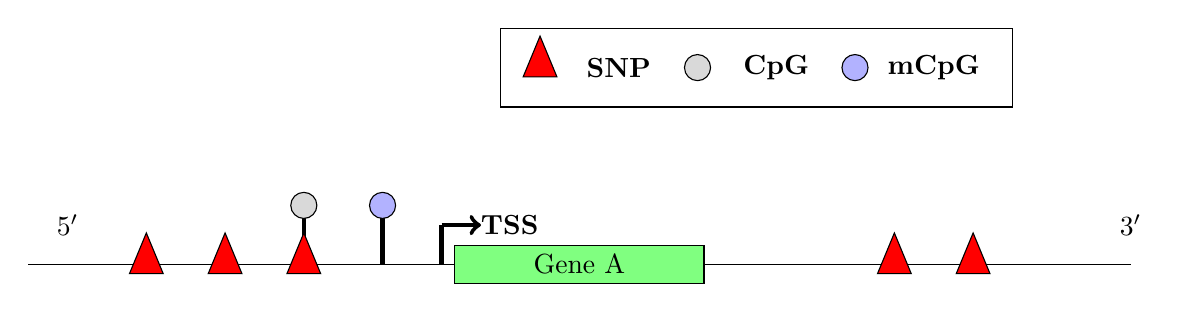
\begin{tikzpicture}[decoration={coil}, dna/.style={decorate, thick, decoration={aspect=0, segment length=0.5cm}}, protein/.style={ellipse, draw=white, minimum width=1cm, minimum height=1cm},
gluon/.style={decorate, thick, decoration={aspect=0, segment length=0.5cm}},cpg/.style={circle, draw=black, minimum width=1mm, minimum height=1mm}]
%DNA
\draw(0,0) -- (14,0);
 %Gene
\node[block1,sharp corners, fill=green!50, inner xsep=20pt] at (7,0) (gene){Gene A};
\draw[ultra thick](5.25,0)--(5.25,0.5);
\draw[ultra thick, ->](5.25,0.5)--(5.75,0.5);
\node[text width=3cm] at (7.25,0.5) {\textbf{TSS}};

%\draw [decorate,decoration={brace,mirror,amplitude=10pt},rotate=+90] (-0.5,-0.5) -- (-0.5,-5.5);

% CpG
\draw[ultra thick](3.5,0)--(3.5,0.75);
\draw[ultra thick](4.5,0)--(4.5,0.75);
\node[cpg,minimum height=2.5mm,fill=gray!30] at (3.5,0.75){};
\node[cpg,minimum height=2.5mm,fill=blue!30] at (4.5,0.75){};

\node at (1.5,0)[isosceles triangle, fill=red,draw=black,rotate=90,minimum size=0.15mm,minimum height=0.15mm](SNP1){};
\node at (2.5,0)[isosceles triangle, fill=red,draw=black,rotate=90,minimum size=0.15mm,minimum height=0.15mm](SNP2){};
\node at (3.5,0)[isosceles triangle, fill=red,draw=black,rotate=90,minimum size=0.15mm,minimum height=0.15mm](SNP2){};
\node at (11,0)[isosceles triangle, fill=red,draw=black,rotate=90,minimum size=0.15mm,minimum height=0.15mm](SNP3){};
\node at (12,0)[isosceles triangle, fill=red,draw=black,rotate=90,minimum size=0.15mm,minimum height=0.15mm](SNP3){};

\node at (6.5,2.5)[isosceles triangle, fill=red,draw=black,rotate=90,minimum size=0.25mm,minimum height=0.25mm](SNP2){};
\node(legend1) at (7.5,2.5){\textbf{SNP}};

\node[cpg,minimum height=2.5mm,fill=gray!30] at (8.5,2.5){};
\node(legend2) at (9.5,2.5){\textbf{CpG }};
\node[cpg,minimum height=2.5mm,fill=blue!30] at (10.5,2.5){};
\node(legend3) at (11.5,2.5){\textbf{mCpG }};
\draw (6,3)--(12.5,3)--(12.5,2)--(6,2)--(6,3);

\node (5p) at (0.5,0.5) {$5^\prime$};
\node (3p) at (14,0.5) {$3^\prime$};

\end{tikzpicture}
%}
\end{center}
\caption[An illustration of the analysis design]{An illustration of the analysis design. The red triangles indicate SNPs and the circles, CpG sites (gray = unmethylated; blue = methylated). CpG sites that are at least 1.5 Kb from the transcription start site (TSS) of a gene were picked for the analysis. All the SNPs that were picked did not exceed 100 kilobase up- and down-stream of the transcription start site of a gene (\emph{cis}-SNPs). }
\end{figure}

Each mRNA-CpG pair will be tested for a strong association with every \emph{cis}-SNP thus identifying significantly associated \underline{mRNA-CpG-SNP triplets}. 

\subsection{Data Preprocessing}
\subsubsection{Gene Expression data}
Gene expression on four brain regions are publicly available (Gene Expression Omnibus (GEO) Accession Number: GSE15745) as rank-invariant \cite{rankInvariant} normalized gene expression data. All the negative values in the gene expression dataset are changed to a 1 and the entire dataset was then log2 transformed. Variance due to tissue source, tissue bank and the hybridization batch were visualized using principal component analysis (PCA). Before generating the PCA plots, samples with African and Asian ancestry were removed from the analysis. All the gene expression probes on sex chromosomes X and Y were removed from the analysis. As evident from the PCA plot, there are four distinct clusters of samples based on tissue source. Tissue bank and hybridization batch do not influence the cluster formation. In order to identify outliers in the PCA analysis, a simple yet standard approach or rule has been adopted. All the samples that did not follow the \emph{'IQR rule'} ($median + 1.5 * IQR$) were excluded from further analysis (one CRBLM, one FCTX and two PONS). These samples were also eliminated by Gibbs \emph{et al} in their original analysis. 

Each gene expression probe was then adjusted for the biological and methodological covariates such as tissue bank, gender, hybridization batch and numeric covariates such as post-mortem interval (PMI) and age in order to remove any associated confounding effects using the following linear model --

\begin{equation*}
Y = \beta_0 + \beta_1 X_1 + \beta_2 X_2 + \ldots + \beta_n X_n + PC_1 + \ldots + PC_{50} + \epsilon
\end{equation*}

where Y is the gene expression data, $X_1 \ldots X_n$ represent the aforementioned biological and methodological covariates while $PC_1 \ldots PC_{50}$ are the top 50 principal components obtained from the original gene expression data. In order to target the difference in the genetic variation of expression among tissues, global variation in expression among tissues was removed by using the residual expression for each probe in each tissue after removing 50 PCs for further downstream analyses. It was shown in the past that the number of \emph{cis-}eQTL detected significantly improved when 50 PCs were removed from the expression data \cite{Fu_Jing}.

\begin{center}
\begin{figure}[!ht]
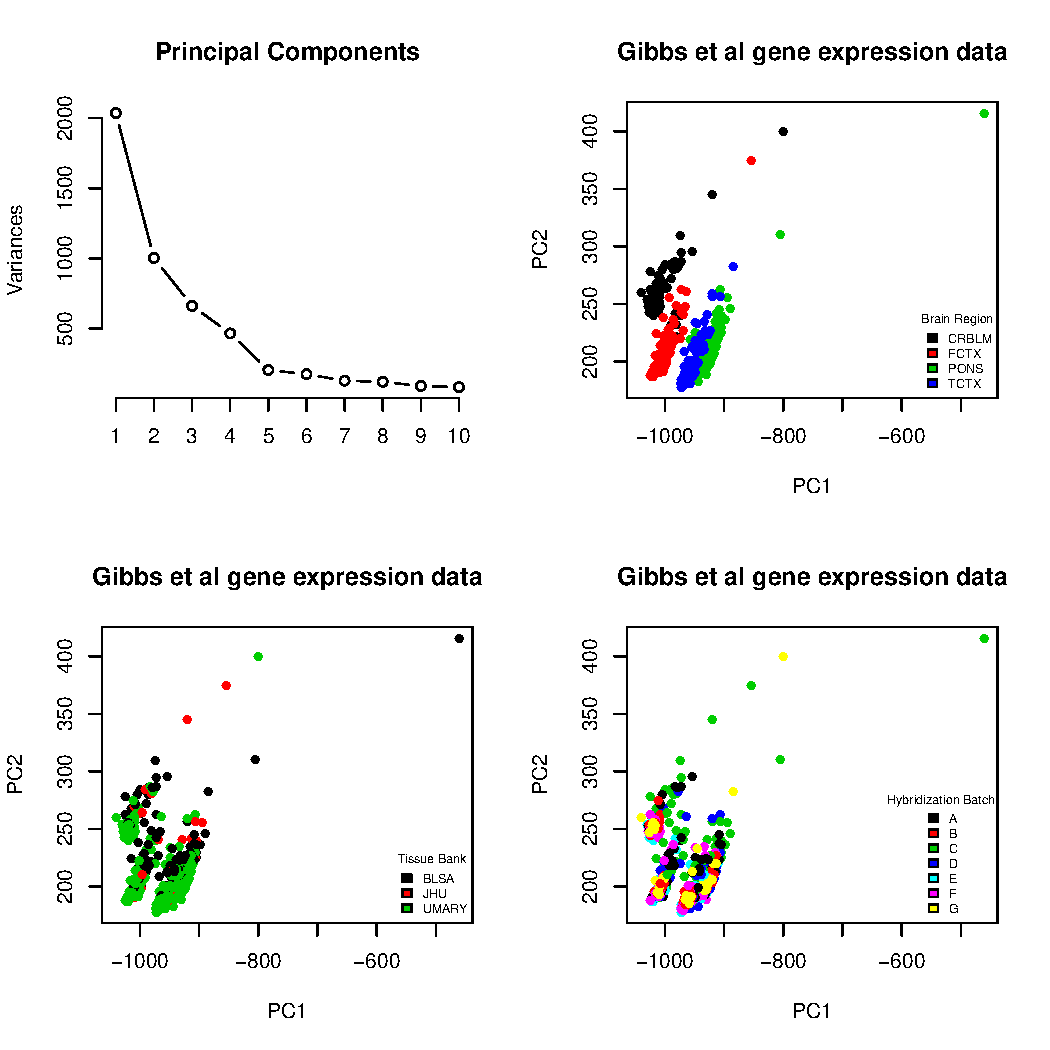
\includegraphics[width=\textwidth]{pca_gene_exp.pdf}
\caption[PCA plots of the gene expression data]{PCA plots exploring the presence of any biological or methodological variation using the first two principal components of the unadjusted rank-invariant normalized gene expression data.}
\end{figure}
\end{center}

\subsubsection{Genotype data}
The genotype data is recoded into a SNP matrix of values 0, 1 and 2 representing minor allele counts. Samples with African and Asian ancestry were removed from the analysis. These SNPs were filtered on the missing-ness of the individual data and the SNP data (excluded SNPs with missing data), followed by MAF (included SNPs with MAF $\geq$ 0.05)and Hardy-Weinberg equilibrium (HWE; p-values $\leq$ 0.001) in the same order using PLINK \cite{Plink} software. SNPs with missing values were removed from the analysis. We ended with 400,097 SNPs after preprocessing. 

\subsubsection{Methylation data}
Methylation data, obtained as a ``series matrix file" from GEO consisted of Beta-values, which represent the ratio of methylated probe intensity and the overall intensity (sum of methylated and unmethylated probe intensities) \cite{Beta-M}. Therefore, Beta value for an $i^{th}$ interrogated CpG site is --

\begin{equation*}
Beta_i = \frac{ max(y_{i,methyl},0) }{max(y_{i,methyl},0) + max(y_{i,unmethyl},0) + const}
\end{equation*}
where $y_{i,methyl}$ and $y_{i,unmethyl}$ are the intensities measured by the $i^{th}$ methylation and unmethylated probes, respectively. Beta values range between 0 and 1. An initial assessment of the methylation data included PCA verification of the presence of any potential confounding variables. The first two principal components plotted as a scattered plot show no visible variation between the frontal and temporal cortices as was observed by the authors \cite{gibbs}. The methylation data was later adjusted for the biological and methodological covariates such as tissue bank, gender, hybridization batch and numeric covariates such as post-mortem interval (PMI) and age in order to remove any associated confounding effects using the following linear model --

\begin{equation*}
Y = \beta_0 + \beta_1 X_1 + \beta_2 X_2 + \ldots + \beta_n X_n + \epsilon
\end{equation*}
where Y is the methylation expression data and $X_1 \ldots X_n$ represent the aforementioned biological and methodological covariates. The residual methylation expression was later used in the subsequent downstream analyses. 

\begin{center}
\begin{figure}[!ht]
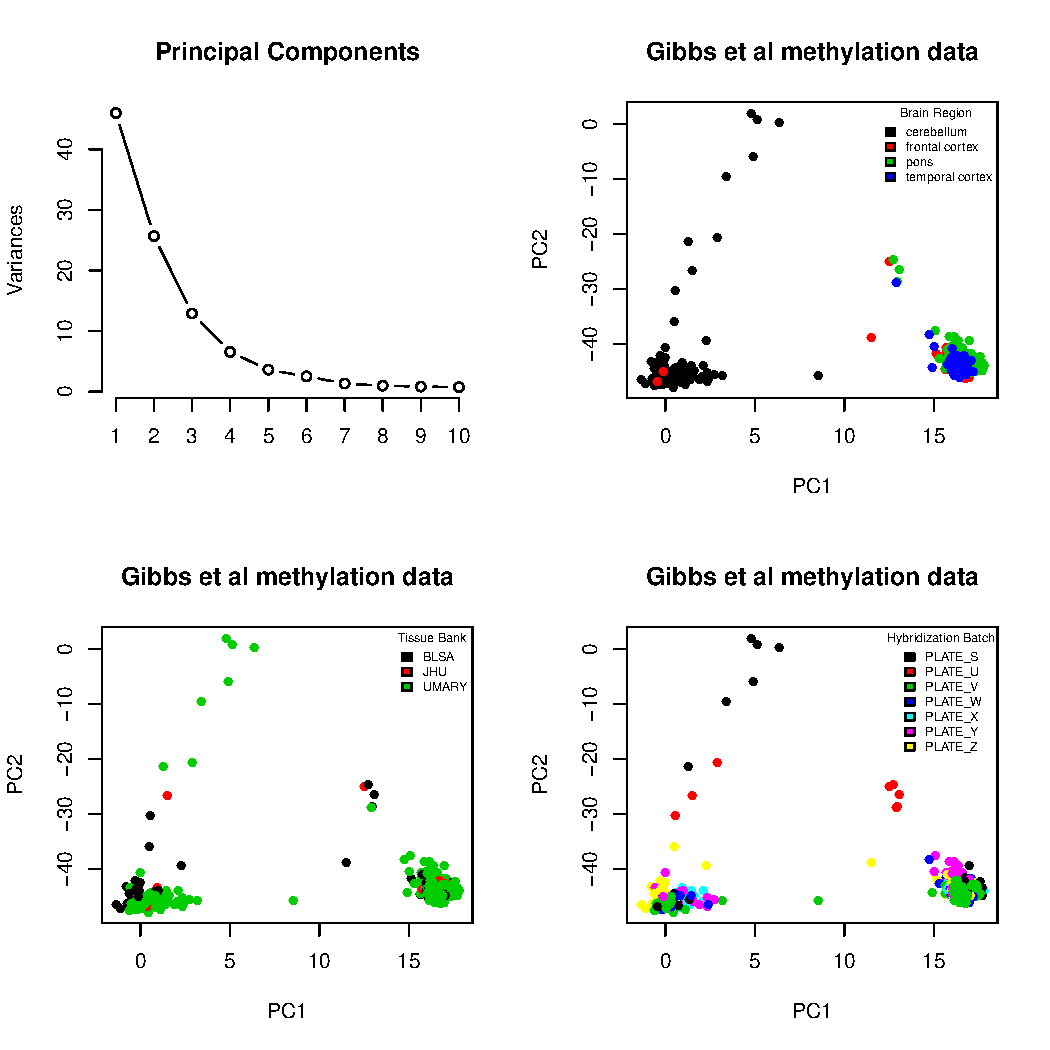
\includegraphics[width=\textwidth]{pca_meth_exp.pdf}
\caption[PCA plots of the methylation data]{PCA plots exploring the presence of any biological or methodological variation using the first two principal components of the unadjusted methylation data.}
\end{figure}
\end{center}

\subsection{Results}
The following different types of analyses were performed --

\begin{itemize}
\item A region-by-region eQTL and mQTL analyses 
\item A region-by-region analysis using a linear model
\item Joint analysis using JAGUAR
\item Joint analysis using our current model
\end{itemize}

\subsubsection{Region-by-Region analysis: Separate eQTL and mQTL analysis}

Currently, this is the most commonly used approach in associating CpG sites, SNPs and genes. Gibbs \emph{et al} have first selected every pairing of CpG methylation sites and mRNA transcripts or genes (CpG site is less than 1 Mb from the transcription start site of a gene) and both the CpG site or the mRNA transcript had a significant \emph{cis}-eQTL. mRNA-CpG-SNP triplets were then identified based on the significant correlations between the \emph{cis}-SNP and either mRNA transcript or the CpG methylation site. We have employed the same strategy. 

A region-by-region eQTL and mQTL analysis was performed using the following additive model --

\begin{equation*}
Y = \beta_0 + \beta_1 G + \epsilon
\end{equation*}
where $Y$ is either gene expression or CpG methylation expression data and $G$ represents genotypes encoded as allele dosage. In order to correct for the number of traits being tested, the $p$~values obtained from the above model were adjusted for multiple hypothesis using an optimized FDR approach \cite{qvalue}. $Q$~values were estimated from each set of $p$~values (originated from each region-by-region analysis) and minimum $q$~value for a given mRNA-SNP or CpG-SNP pair across all the brain regions was computed, which indicates the presence of a statistically significant pair in at least one brain region. The number of significant associations in at least one brain region were then assessed at 5\% FDR ($p$~value $\leq \frac{0.05}{4}$ where 4 is the number of brain regions). 

Using the above process, we identified a total of 11,014 mRNA-\emph{cis}SNP pairs and a total of 3,467 CpG-\emph{cis}SNP pairs significant in at least one region of the brain. Table below indicates the number of mRNA-SNP and CpG-SNP pairs in each brain region. For each mRNA transcript, we selected a CpG site that is at least 1 Mb from the transcription start site (TSS) and both the CpG site and the mRNA transcript had a statistically significant \emph{cis-}eQTL. These mRNA-CpG pairs were expanded to mRNA-CpG-SNP triplets where the SNP was significantly correlated with either the CpG methylation site or the mRNA transcript of the mRNA-CpG pair. We identified a total of 1,928 mRNA-CpG-SNP triplets in at least one brain region. 

\begin{table}[!ht]
\begin{center}
\begin{tabular}{| c | c | c | c | c | c |}
\hline
& CRBLM & FCTX & PONS & TCTX & Common\\ \hline \hline
mRNA - \emph{cis}SNP pairs & 9,556 & 8,957 & 6,373 & 8,683 & 2,481 \\ \hline
CpG - \emph{cis}SNP pairs & 865 & 2,661 & 1,998 & 3,670 & 336 \\
\hline\hline
\end{tabular}
\end{center}
\caption{A region-by-region \emph{cis} analysis of Gibbs \emph{et al} data at a nominal $p$~value of 0.05}
\end{table}

This ad-hoc way of identifying triplets (given the discrepancy in the number of statistically significant CpG-SNP and mRNA-SNP pairs) could be inefficient 

%\begin{table}[!ht]
%\begin{center}
%\resizebox{\linewidth}{!}{
%\begin{tabular}{| c | c | c | c | c | c | c | c | c | c |}
%\hline
%Triplets & Gene & Chromosome & CRBLM & FCTX & PONS & TCTX & SNP Location & CpG Start Location & CpG End Location \\ \hline \hline

%\hline\hline
%\end{tabular}
%}
%\end{center}
%\caption{A list of meQTL as identified by the TBT method. TRUE indicates statistical significance ($q$~value $\leq$ 0.05) whereas FALSE indicates otherwise. Each triplet consists of a mRNA-CpG-SNP combination.}
%\end{table}
%
%We found 12 SNPs located in the CpG island, called meQTL (Table 5).  These meQTL change the methylation status of the CpG site and thus regulate gene expression. 

%\begin{center}
%\begin{figure}[H]
%\includegraphics[width=\textwidth]{triplets.pdf}
%\caption{Heatmap of 1,911 unique mRNA-CpG-SNP triplets in each of the four brain regions. Red indicates statistical significance ($q$~value $\leq$ 0.05) and White indicates the lack thereof. Color bar on the left indicates chromosomes with each color representing each chromosome. Chromosomes are ordered from 1 through 22.}
%\end{figure}
%\end{center}

\subsubsection{Region-by-Region analysis: Identifying triplets using a linear model}

In a region-by-region analysis, we apply the following regression model to identify mRNA-CpG-SNP triplets --

\begin{equation*}
Y = G \beta + M \lambda + MG \phi + \epsilon
\end{equation*}
where $Y$ is the gene expression data, $G$ represents genotypes encoded as allele dosage, $M$ represents CpG methylation expression data and $MG$ represents the interaction effect between a SNP and a CpG site. In order to correct for the number of traits being tested, the $p$~values obtained from the above model were adjusted for multiple hypothesis using an optimized FDR approach \cite{qvalue}. $Q$~values were estimated from each set of $p$~values (originated from each region-by-region analysis) and minimum $q$~value for a given mRNA-SNP or CpG-SNP pair across all the brain regions was computed, which indicates the presence of a statistically significant pair in at least one brain region. The number of significant associations in at least one brain region were then assessed at 5\% FDR ($p$~value $\leq \frac{0.05}{4}$ where 4 is the number of brain regions). 

\begin{table}[!ht]
\begin{center}
\begin{tabular}{| c | c | c | c | c | c |}
\hline
& CRBLM & FCTX & PONS & TCTX & Common\\ \hline \hline
mRNA - CpG - SNP triplets & 8,483 & 9,901 & 5,901 & 7,831 & 1,993\\
\hline\hline
\end{tabular}
\end{center}
\caption{Triplets identified using a region-by-region \emph{cis} analysis of Gibbs \emph{et al} data at a nominal $p$~value of 0.05}
\end{table}

We found 10,926 mRNA-CpG-SNP triplets to be statistically significant in at least one brain region. Out of these, a total of 1,993 triplet associations were found in all four brain regions.

%\begin{table}[!ht]
%\begin{center}
%\resizebox{\linewidth}{!}{
%\begin{tabular}{| c | c | c | c | c | c | c | c | c | c |}
%\hline
%Triplets & Gene & CRBLM & FCTX & PONS & TCTX & Chromosome & SNP Location & CpG Start Location & CpG End Location  \\ \hline \hline

%\hline\hline
%\end{tabular}
%}
%\end{center}
%\caption{meQTL identified using a region-by-region \emph{cis} analysis of Gibbs \emph{et al} data. TRUE indicates statistical significance ($q$~value $\leq$ 0.05) whereas FALSE indicates otherwise. Each triplet consists of a mRNA-CpG-SNP combination.}
%\end{table}

\subsubsection{Joint analysis using JAGUAR}

JAGUAR \cite{jaguar,jaguar_cran} applies the following linear model --

\begin{equation*}
Y = J\alpha + G\beta + Au + Bv  + \xi \qquad \xi \sim N\left(0, \epsilon \right)
\end{equation*}

where $Y$ is the gene expression data, $G$ represents genotypes encoded as allele dosage. If $T$ indicates tissue, the $G \times T$ effect is measured by the random effect $v \sim N\left(0,\gamma \right)$. In order to correct for the number of traits being tested, the $p$~values obtained from the above model were adjusted for multiple hypothesis using an optimized FDR approach \cite{qvalue}.  $Q$~values were estimated from each set of $p$~values (originated from each region-by-region analysis) and minimum $q$~value for a given mRNA-SNP or CpG-SNP pair across all the brain regions was computed, which indicates the presence of a statistically significant pair in at least one brain region. The number of significant associations in at least one brain region were then assessed at 5\% FDR ($p$~value $\leq \frac{0.05}{4}$ where 4 is the number of brain regions). 

JAGUAR was applied to separately identify mRNA-SNP pairs and CpG-SNP pairs following which, these mRNA-CpG pairs were expanded to mRNA-CpG-SNP triplets where the SNP was significantly correlated with either the CpG methylation site or the mRNA transcript of the mRNA-CpG pair. JAGUAR is a score-test based approach that jointly models all the tissues and makes use of all the information available to maximize the power of eQTL mapping. We identified 16,919 mRNA-SNP pairs (96\% overlap with a region-by-region approach) and 4,804 CpG-SNP pairs (91\% overlap with a region-by-region approach) significant in at least one region of the brain. For each mRNA transcript, we selected a CpG site that is at least 1 Mb from the transcription start site (TSS) and both the CpG site and the mRNA transcript had a statistically significant \emph{cis-}eQTL. These mRNA-CpG pairs were expanded to mRNA-CpG-SNP triplets where the SNP was significantly correlated with either the CpG methylation site or the mRNA transcript of the mRNA-CpG pair. We identified a total of 1,095 mRNA-CpG-SNP triplets in at least one brain region. 

\subsubsection{Joint analysis using our current model}

We applied our joint model --

\begin{equation*}
Y = J\alpha + G\beta + M\lambda + MG\phi + Au + Bv + Cw + Dx + \xi	\qquad \xi \sim N\left(0, \epsilon \right)
\end{equation*}

where $Y$ is the gene expression data, $G$ represents genotypes encoded as allele dosage, $M$ represents CpG methylation expression data and $MG$ represents the interaction effect between a SNP and a CpG site. If $T$ indicates tissue, the $G \times T$ effect is measured by the random effect $v \sim N\left(0,\gamma \right)$, the $G \times T \times M$ effect is measured by $w \sim N\left(0,\delta\right)$. In order to correct for the number of traits being tested, the $p$~values obtained from the above model were adjusted for multiple hypothesis using an optimized FDR approach \cite{qvalue}.  $Q$~values were estimated from each set of $p$~values and we computed the minimum $q$~value for mRNA-CpG-SNP triplets. The number of significant associations were then assessed at 5\% FDR ($p$~value $\leq 0.05$). 

%\begin{landscape}
%\small
%%\begin{longtable}{ l l l l l l }
%\setlength\LTleft{0pt}            % default: \parindent
%\setlength\LTright{0pt}           % default: \fill
%\begin{longtable}{@{\extracolsep{\fill}}|*{6}{c |}}
%\hline
%Triplets & Gene & Chromosome & SNP Location & CpG Start Location & CpG End Location  \\ \hline \hline
%\endfirsthead
%Triplets & Gene & Chromosome & SNP Location & CpG Start Location & CpG End Location  \\ \hline \hline
%\endhead
%\multicolumn{6}{r}{{Continued\ldots}} \
%\endfoot
%\hline
%\endlastfoot

%\hline \hline
%\caption{A list of 62 meQTL as identified by our joint score test approach. Triplets of mRNA-CpG-SNP in bold were identified by a region-by-region analysis. A total of 18 (out of 19) triplets were picked up by our method. }
%\end{longtable}
%\end{landscape}

When applied our joint model on Gibbs \emph{et al} data, we identified 13,212 statistically significant mRNA - CpG - SNP triplets with approximately 75\% overlap with the number of triplets identified by the region-by-region analysis. 

%\begin{figure}[!ht]
%\hfill
%\subfigure[8,555 statistically significant triplets ]{\includegraphics[width=8.5cm]{JT_stat_plot.pdf}}
%\hfill
%\subfigure[62 meQTL]{\includegraphics[width=8cm]{meQTL_plot.pdf}}
%\hfill
%\caption[Plotting triplets identified by our joint analysis]{Triplets with expanded statistics. All the values are -log10 unadjusted $p$~values of individual statistics that comprise our joint score test statistic. }
%\end{figure}

\begin{table}[H]
\begin{center}
\begin{tabular}{| c | c | c | c | c |}
\hline
$p~value \leq 0.05$ & $U_\beta$ & $U_\phi$ & $U_\gamma$ & $U_\delta$ \\ \hline \hline
TRUE & 11,994 (90.8\%) &  1,140 (8.6\%) & 11,036 (83.5\%) & 1,985 (15\%) \\ \hline
FALSE & 1,218 (9.2\%) & 12,072 (91.4\%) & 2,176 (16.5\%) & 11,227 (85\%) \\ \hline
\hline\hline
\end{tabular}
\end{center}
\caption{The distribution of the different types of effects as measured by our joint score test statistic. $U_\beta$ is a measure of the main additive genetic effect. $U_\phi$ is a measure of $G \times M$ effect. $U_\gamma$ measures $G \times T$ effect while $U_\delta$ is a measure of $G \times M \times T$.}
\end{table}

Our joint score test method identifies mRNA-CpG-SNP associations 	that weren't picked up by either a region-by-region method or by JAGUAR. For example, DiGeorge Syndrome Critical Region Gene 8 (DGCR8; ILMN1694223) was identified to be significantly associated with CpG site cg18251360 and SNP rs10212087 using our joint method. DGCR8, found on chromosome 22, was previously implicated in schizophrenia \cite{dgcr}. This association was not picked up by any of the other methods. 

\begin{center}
\begin{figure}[H]
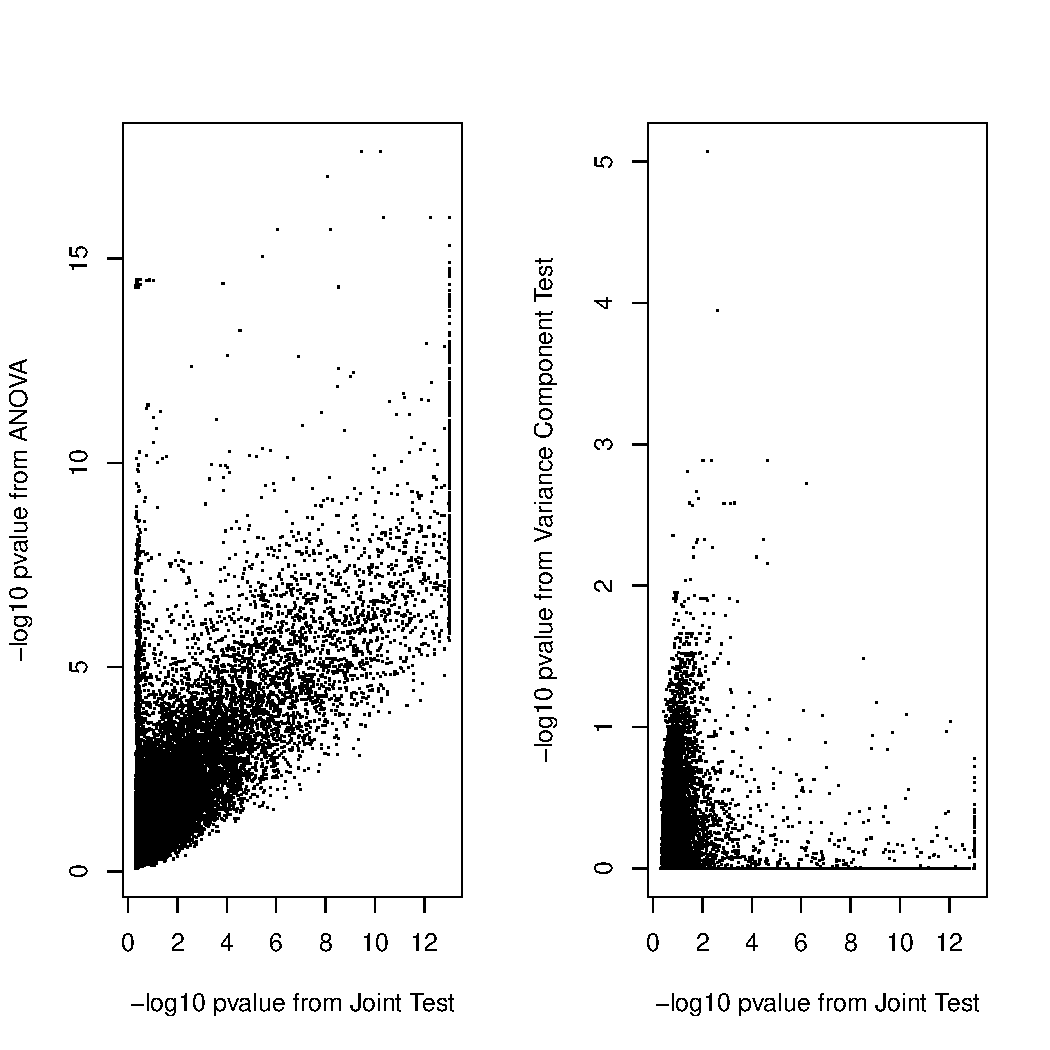
\includegraphics[width=\textwidth]{jt_plots.pdf}
\caption{Scatter plot of -log10 $p$~values from our joint score test and both a region-by-region analysis and $G \times M \times T$ variance component score test, $\ddot{U_\delta}$}
\end{figure}
\end{center}

\section{Conclusions}

Our method investigates the presence of a number of genetic and epigenetic effects: 1) an overall shift in gene expression due to genotypes, 2) an overall shift in gene expression due to interaction between genotypes and CpG site methylation, 3) tissue-specific effects of genotypes,  and 4) tissue-specific effects of combined methylation and genotypes on gene expression. Our approach models tissue-specific effects and tissue-specific interaction between genotype and methylation as random effects, resulting in an efficient test for identifying statistically significant association between a given mRNA-CpG-SNP triplet. Currently, there are no methods that jointly model the epigenetic and genetic effects of tissue-specific gene expression. 

An expression quantitative trait loci (eQTL) study focuses on identifying genetic variants that are correlated with gene expression in one or more genes. However, in the presence of epigenetic elements such as CpG island methylation that negatively affects gene expression, many eQTL studies fail to 

The dataset examined here used genome-wide association study (GWAS) SNP array platform to interrogate germ-line variation that include an overwhelming number of common variants. 

\section{Mathematical derivations}

\begingroup
\large
\begin{equation}
\textbf{Y} = J \alpha + G\beta + Au + Bv + Cw + Dx  + \xi
\end{equation}
\endgroup

where --

\begin{itemize}
\large
\item \textbf{Y} is \emph{$nt \times 1$} vector, and $Y_i = \left(Y_{i1}, Y_{i2}, \cdots , Y_{it} \right)^T$
\item $\boldsymbol{\xi} = \left( \xi_i^T, \cdots , \xi_n^T \right)^T$ is a \emph{$nt \times 1$} vector
\item $\boldsymbol{J} = \left( I_t, \cdots , I_t \right)^T$ is a $nt \times t$ matrix
\item $\boldsymbol{\alpha} =\left( \alpha_1, \alpha_2, \cdots , \alpha_t \right)^T$ is a vector of length $t$
\item \textbf{G} is $nt \times 1$ vector and $G_i = \left(G_{i1}, G_{i2}, \cdots , G_{it} \right)^T$
\item \textbf{A} is $nt \times n$ model matrix with each column represented by a combination of $1_t^T$ and \textbf{zeros} indicating an individual's intercept. 
\item \textbf{u} is a vector of individual-specific random effects of length $n$.
\item \textbf{B}$=\left(g_i I_t, \cdots , g_n I_t \right)^T$ is a $nt \times t$ matrix
\item \textbf{v}$=\left(v_1, v_2, \cdots, v_t\right)^T$ is a vector of length $t$ and $v \sim N_t \left(0, \gamma \right)$
\item \textbf{C}$=\left(g_i M_t, \cdots , g_n M_t \right)^T$ is a $nt \times t$ matrix
\item \textbf{w}$=\left(w_1, w_2, \cdots, w_t\right)^T$ is a vector of length $t$ and $w_{t} \sim N_t \left(0, \delta \right)$
\item \textbf{D}$=\left( M_t, \cdots, M_t \right)^T$ is a $nt \times t$ matrix
\item \textbf{x}$=\left(x_1, x_2, \cdots, x_t\right)^T$ is a vector of length $t$ and $x_t \sim N_t \left(0, \theta \right)$
\end{itemize}

Parameters of interest --

\[
\Large
\Theta = \left\{ \gamma, \delta \right\} \quad and \quad \beta \quad and \quad \phi
\]

We define global null as --

\begingroup
\large
\begin{center}
$
\boxed{
H_0: \beta = \phi = \Theta = 0; \qquad H_A: \beta \neq 0; \phi \neq 0; \quad \Theta > 0
}
$
\end{center}
\endgroup

From equation 1, the likelihood function of Y conditioned on the genotype can be written as --

\begin{equation}
L_n\left( \Theta; Y \right) = \prod\limits_{i=1}^n \left( 2 \pi \right) ^{-\frac{n}{2}} \mid \Sigma_{i} \mid ^{-\frac{1}{2}} exp \left[ -\frac{1}{2} \left( Y  - J \alpha -  G\beta - M\lambda - MG\phi \right)^T \Sigma_{i}^{-1} \left( Y  - J \alpha -  G\beta - M\lambda - MG\phi \right) \right]
\end{equation}

The marginal log-likelihood function derived from the above equation is --

\begin{equation}
\ell_n\left( \Theta ;Y \right) =  - c - \frac{1}{2} \log \mid \Sigma \mid - \frac{1}{2} \left( Y  - J \alpha - G\beta - M\lambda - MG\phi \right )^T \Sigma ^{-1} \left( Y  - J \alpha - G\beta - M\lambda - MG\phi \right )
\end{equation}

In other words, the marginal distribution of the above model can be represented as --

\[
Y \sim N( J\alpha + G\beta + M\lambda + MG\phi,\Sigma )
\]

where $\Sigma$ is the total variance for an individual. Variance for a single individual looks like a $t \times t$ matrix of $\epsilon$, $\tau$, $\gamma$, $\delta$, $\phi$ and $\theta$ where $t$ is the number of tissues. In a matrix format, for all individuals the total variance can be represented as  --

\begin{center}
$
\boxed{
\Sigma_{n}  = \epsilon I_n + \tau A A^{T} + \gamma B B^{T} + \delta C C^T + \theta D D^T 
}
$
\end{center}

While $AA^T$ forms a block diagonal structure whereas $BB^T$, $CC^T$ and $DD^T$ do not. Model matrix $B$ is a function of genotype while $C$ is a function of both genotype and methylation data. $D$ is a function of just the methylation data. 

\subsection{Score function}

\begingroup
\large
\begin{equation*}
\frac{\partial \ell_i }{\partial \alpha} = \Sigma_i^{-1} \left(y_{i,j}-\alpha_{j}- \textbf{1}_t \beta_j g_i - \lambda_j m_{i} - \phi_j m_{i}g_i\right)
\end{equation*}
\endgroup

\begingroup
\large
\begin{equation*}
\frac{\partial \ell_i }{\partial \beta} =  \textbf{1}_t g_i\Sigma_i^{-1} \left(y_{i,j}-\alpha_{j}- \textbf{1}_t \beta_j g_i - \lambda_j m_{i} -  \phi_j m_{i}g_i\right)
\end{equation*}
\endgroup

\begingroup
\large
\begin{equation*}
\frac{\partial \ell_i }{\partial \lambda} =  \textbf{1}_t m_{i}\Sigma_i^{-1} \left(y_{i,j}-\alpha_{j}- \textbf{1}_t \beta_j g_i - \lambda_j m_{i} -  \phi_j m_{i}g_i\right)
\end{equation*}
\endgroup

\begingroup
\large
\begin{equation*}
\frac{\partial \ell_i }{\partial \phi} =   m_{i}g_i \Sigma_i^{-1} \left(y_{i,j}-\alpha_{j}- \textbf{1}_t \beta_j g_i - \lambda_j m_{i} -  \phi_j m_{i}g_i\right)
\end{equation*}
\endgroup


\begingroup
\large
\begin{equation*}
\begin{split}
\frac{\partial \ell_i }{\partial \tau} &= \frac{1}{2} \left\{ \left(y_{i,j}-\alpha_{j}-\textbf{1}_t \beta_j g_i - \lambda_j m_i \right)^T \Sigma_i^{-1} \frac{\partial \Sigma_i }{\partial \tau}\Sigma_i^{-1} \left(y_{i,j}-\alpha_{j}-\textbf{1}_t \beta_j g_i- \lambda_j m_i \right) - \Tr \left( \Sigma_i^{-1}  \frac{\partial \Sigma_i }{\partial \tau}\right) \right\}\\
&=\frac{1}{2} \left\{ \left(y_{i,j}-\alpha_{j}-\textbf{1}_t \beta_j g_i - \lambda_j m_i\right)^T \Sigma_i^{-1} A_i A_i^T \Sigma_i^{-1}  \left(y_{i,j}-\alpha_{j}-\textbf{1}_t \beta_j g_i - \lambda_j m_i\right) - \Tr \left( \Sigma_i^{-1}  A_i A_i^T\right) \right\} \\
\end{split}
\end{equation*}
\endgroup

\begingroup
\large
\begin{equation*}
\begin{split}
\frac{\partial \ell_i }{\partial \gamma} &= \frac{1}{2} \left\{ \left(y_{i,j}-\alpha_{j}-\textbf{1}_t \beta_j g_i- \lambda_j m_i\right)^T \Sigma_i^{-1} \frac{\partial \Sigma_i }{\partial \gamma}\Sigma_i^{-1} \left(Y_{i,j}-\alpha_{j}-\textbf{1}_t \beta_j g_i - \lambda_j m_i \right) - \Tr \left( \Sigma_i^{-1}  \frac{\partial \Sigma_i }{\partial \gamma}\right) \right\}\\
&=\frac{1}{2} \left\{ \left(y_{i,j}-\alpha_{j}-\textbf{1} \beta_j g_i - \lambda_j m_i\right)^T \Sigma_i^{-1} B_iB_i^T \Sigma_i^{-1}  \left(y_{i,j}-\alpha_{j}-\textbf{1}_t \beta_j g_i - \lambda_j m_i\right) - \Tr \left( \Sigma_i^{-1}  B_iB_i^T\right) \right\} \\
\end{split}
\end{equation*}
\endgroup

\begingroup
\large
\begin{equation*}
\begin{split}
\frac{\partial \ell_i }{\partial \delta} &= \frac{1}{2} \left\{ \left(y_{i,j}-\alpha_{j}-\textbf{1}_t \beta_j g_i - \lambda_j m_i\right)^T \Sigma_i^{-1} \frac{\partial \Sigma_i }{\partial \delta}\Sigma_i^{-1} \left(Y_{i,j}-\alpha_{j}-\textbf{1}_t \beta_j g_i - \lambda_j m_i\right) - \Tr \left( \Sigma_i^{-1}  \frac{\partial \Sigma_i }{\partial \delta}\right) \right\}\\
&=\frac{1}{2} \left\{ \left(y_{i,j}-\alpha_{j}-\textbf{1} \beta_j g_i - \lambda_j m_i\right)^T \Sigma_i^{-1} C_iC_i^T \Sigma_i^{-1}  \left(y_{i,j}-\alpha_{j}-\textbf{1}_t \beta_j g_i - \lambda_j m_i \right) - \Tr \left( \Sigma_i^{-1}  C_iC_i^T\right) \right\} \\
\end{split}
\end{equation*}
\endgroup

\begingroup
\large
\begin{equation*}
\begin{split}
\frac{\partial \ell_i }{\partial \theta} &= \frac{1}{2} \left\{ \left(y_{i,j}-\alpha_{j}-\textbf{1}_t \beta_j g_i - \lambda_j m_i \right)^T \Sigma_i^{-1} \frac{\partial \Sigma_i }{\partial \theta}\Sigma_i^{-1} \left(Y_{i,j}-\alpha_{j}-\textbf{1}_t \beta_j g_i- \lambda_j m_i \right) - \Tr \left( \Sigma_i^{-1}  \frac{\partial \Sigma_i }{\partial \theta}\right) \right\}\\
&=\frac{1}{2} \left\{ \left(y_{i,j}-\alpha_{j}-\textbf{1} \beta_j g_i - \lambda_j m_i\right)^T \Sigma_i^{-1} E_i E_i^T \Sigma_i^{-1}  \left(y_{i,j}-\alpha_{j}-\textbf{1}_t \beta_j g_i - \lambda_j m_i\right) - \Tr \left( \Sigma_i^{-1}  E_i E_i^T\right) \right\} \\
\end{split}
\end{equation*}
\endgroup

\begingroup
\large
\begin{equation*}
\begin{split}
\frac{\partial \ell_i }{\partial \epsilon} &= \frac{1}{2} \left\{ \left(y_{i,j}-\alpha_{j}-\textbf{1}_t \beta_j g_i - \lambda_j m_i\right)^T \Sigma_i^{-1} \frac{\partial \Sigma_i }{\partial \epsilon}\Sigma_i^{-1} \left(y_{i,j}-\alpha_{j,t}-\textbf{1}_t \beta_j g_i - \lambda_j m_i\right) - \Tr \left( \Sigma^{-1}  \frac{\partial V_i }{\partial \epsilon}\right) \right\}\\
&=\frac{1}{2} \left\{ \left(y_{i,j}-\alpha_{j}-\textbf{1}_t \beta_j g_i - \lambda_j m_i\right)^T \Sigma_i^{-1} I \Sigma_i^{-1}  \left(y_{i,j}-\alpha_{j}-\textbf{1}_t \beta_j g_i - \lambda_j m_i\right) - \Tr \left( \Sigma_i^{-1} I\right) \right\}\\
&=\frac{1}{2} \left\{ \left(y_{i,j}-\alpha_{j}-\textbf{1}_t \beta_j g_i - \lambda_j m_i\right)^T \Sigma_i^{-2} \left(y_{i,j}-\alpha_{j}-\textbf{1}_t \beta_j g_i - \lambda_j m_i\right) - \Tr \left( \Sigma_i^{-1}\right) \right\}
\end{split}
\end{equation*}
\endgroup

\subsection{Information matrix}

\begingroup
\large
\begin{equation*}
\begin{split}
I_{\beta\alpha} &= - E_{Y|G=g}\left[ \frac{\partial^2 \ell_i }{\partial \beta \partial \alpha}\right]\\
&= \Sigma_i^{-1} E[g_i] \\
&= \Sigma_i^{-1} \sum\limits_{i=1}^n g_i
\end{split}
\end{equation*}
\endgroup

\begingroup
\large
\begin{equation*}
\begin{split}
I_{\beta\lambda} &= - E_{Y|G=g}\left[ \frac{\partial^2 \ell_i }{\partial \beta \partial \lambda}\right]\\
&= \Sigma_i^{-1} \sum\limits_{i=1}^n m_i g_i
\end{split}
\end{equation*}
\endgroup

\begingroup
\large
\begin{equation*}
\begin{split}
I_{\alpha\alpha} &= - E_{Y|G=g}\left[ \frac{\partial^2 \ell_i }{\partial \alpha \partial \alpha^T}\right]\\
&= \Sigma_i^{-1}
\end{split}
\end{equation*}
\endgroup

\begingroup
\large
\begin{equation*}
\begin{split}
I_{\alpha\lambda} &= - E_{Y|G=g}\left[ \frac{\partial^2 \ell_i }{\partial \alpha \partial \lambda}\right]\\
&= \Sigma_i^{-1}  \sum\limits_{i=1}^n m_i
\end{split}
\end{equation*}
\endgroup

\begingroup
\large
\begin{equation*}
\begin{split}
I_{\lambda\lambda} &= - E_{Y|G=g}\left[ \frac{\partial^2 \ell_i }{\partial \lambda \partial \lambda^T}\right]\\
&= \Sigma_i^{-1}  \sum\limits_{i=1}^n g_i m_i^2
\end{split}
\end{equation*}
\endgroup


\begingroup
\large
\begin{equation*}
\begin{split}
I_{\gamma\tau} &= - E_{Y|G=g}\left[ \frac{\partial^2 \ell_i }{\partial \gamma \partial \tau}\right]\\
&= - \left(-\frac{1}{2} \Tr\left(V^{-1}\frac{\partial \Sigma_i }{\partial \gamma} \Sigma_i^{-1}\frac{\partial \Sigma_i }{\partial \tau} \right) \right)\\
&= \frac{1}{2} \Tr \left(\Sigma_i^{-1} B_i B_i^T \Sigma_i^{-1} A_i A_i^T \right)\\
\end{split}
\end{equation*}
\endgroup

\begingroup
\large
\begin{equation}
\begin{split}
I_{\gamma\epsilon} &= - E_{Y|G=g}\left[ \frac{\partial^2 \ell_i }{\partial \gamma \partial \epsilon}\right]\\
&= - \left(-\frac{1}{2} \Tr\left(\Sigma_i^{-1}\frac{\partial \Sigma_i }{\partial \gamma} \Sigma_i^{-1}\frac{\partial \Sigma_i }{\partial \epsilon} \right) \right)\\
&= \frac{1}{2} \Tr \left(\Sigma_i^{-1} B_i B_i^T \Sigma_i^{-1}I \right)\\
\end{split}
\end{equation}
\endgroup

\begingroup
\large
\begin{equation*}
\begin{split}
I_{\delta\tau} &= - E_{Y|G=g}\left[ \frac{\partial^2 \ell_i }{\partial \delta \partial \tau}\right]\\
&= - \left(-\frac{1}{2} \Tr\left(\Sigma^{-1}\frac{\partial \Sigma_i }{\partial \delta} \Sigma_i^{-1}\frac{\partial \Sigma_i }{\partial \tau} \right) \right)\\
&= \frac{1}{2} \Tr \left(\Sigma_i^{-1} C_i C_i^T \Sigma_i^{-1} A_i A_i^T \right)\\
\end{split}
\end{equation*}
\endgroup

\begingroup
\large
\begin{equation}
\begin{split}
I_{\delta\epsilon} &= - E_{Y|G=g}\left[ \frac{\partial^2 \ell_i }{\partial \gamma \partial \epsilon}\right]\\
&= - \left(-\frac{1}{2} \Tr\left(\Sigma_i^{-1}\frac{\partial \Sigma_i }{\partial \delta} \Sigma_i^{-1}\frac{\partial \Sigma_i }{\partial \epsilon} \right) \right)\\
&= \frac{1}{2} \Tr \left(\Sigma_i^{-1} C_i C_i^T \Sigma_i^{-1}I \right)\\
\end{split}
\end{equation}
\endgroup

\begingroup
\large
\begin{equation*}
\begin{split}
I_{\phi\tau} &= - E_{Y|G=g}\left[ \frac{\partial^2 \ell_i }{\partial \phi \partial \tau}\right]\\
&= - \left(-\frac{1}{2} \Tr\left(\Sigma^{-1}\frac{\partial \Sigma_i }{\partial \gamma} \Sigma_i^{-1}\frac{\partial \Sigma_i }{\partial \tau} \right) \right)\\
&= \frac{1}{2} \Tr \left(\Sigma_i^{-1} D_i D_i^T \Sigma_i^{-1} A_i A_i^T \right)\\
\end{split}
\end{equation*}
\endgroup

\begingroup
\large
\begin{equation}
\begin{split}
I_{\phi\epsilon} &= - E_{Y|G=g}\left[ \frac{\partial^2 \ell_i }{\partial \gamma \partial \epsilon}\right]\\
&= - \left(-\frac{1}{2} \Tr\left(\Sigma_i^{-1}\frac{\partial \Sigma_i }{\partial \gamma} \Sigma_i^{-1}\frac{\partial \Sigma_i }{\partial \epsilon} \right) \right)\\
&= \frac{1}{2} \Tr \left(\Sigma_i^{-1} D_i D_i^T \Sigma_i^{-1}I \right)\\
\end{split}
\end{equation}
\endgroup

\begingroup
\large
\begin{equation}
\begin{split}
I_{\tau\tau} &= - E_{Y|G=g}\left[ \frac{\partial^2 \ell_i }{\partial \tau \partial \tau^T}\right]\\
&= - \left(-\frac{1}{2} \Tr\left(V_i^{-1}\frac{\partial \Sigma_i }{\partial \tau} \Sigma_i^{-1}\frac{\partial \Sigma_i }{\partial \tau} \right) \right)\\
&= \frac{1}{2} \Tr \left(\Sigma_i^{-1} A_i A_i^T \Sigma_i^{-1} A_i A_i^T\right)\\
\end{split}
\end{equation}
\endgroup

\begingroup
\large
\begin{equation}
\begin{split}
I_{\tau\epsilon} &= - E_{Y|G=g}\left[ \frac{\partial^2 \ell_i }{\partial \tau \partial \epsilon}\right]\\
&= - \left(-\frac{1}{2} \Tr\left(\Sigma_i^{-1}\frac{\partial \Sigma_i }{\partial \tau} \Sigma_i^{-1}\frac{\partial \Sigma_i }{\partial \epsilon} \right) \right)\\
&= \frac{1}{2} \Tr \left(\Sigma_i^{-1} A_i A_i^T \Sigma_i^{-1}\right)\\
\end{split}
\end{equation}
\endgroup

\begingroup
\large
\begin{equation}
\begin{split}
I_{\epsilon\epsilon} &= - E_{Y|G=g}\left[ \frac{\partial^2 \ell_i }{\partial \epsilon \partial \epsilon}\right]\\
&= - \left(-\frac{1}{2} \Tr\left(\Sigma_i^{-1}\frac{\partial \Sigma_i }{\partial \epsilon} \Sigma_i^{-1}\frac{\partial \Sigma_i }{\partial \epsilon} \right) \right)\\
&= \frac{1}{2} \Tr \left(\Sigma_i^{-1} I \Sigma_i^{-1}I\right)\\
&= \frac{1}{2} \Tr \left(\Sigma_i^{-2} \right)\\
\end{split}
\end{equation}
\endgroup

%
\subsection{Joint score test}
%
Let the \underline{parameters of interest} be $\psi = (\beta, \phi, \gamma, \delta)^T$ and the \underline{nuisance parameters} be $\eta = (\alpha, \lambda, \tau, \theta, \epsilon)^T$. The following is constructed under the null ($H_0$) --

\[
\large
U_{\psi} = \begin{bmatrix}\frac{\partial l }{\partial \beta} \\ \frac{\partial l }{\partial \phi} \\ \frac{\partial l }{\partial \gamma} \\  \frac{\partial l }{\partial \delta}  \end{bmatrix}
 - \begin{bmatrix} I_{\beta\alpha} & I_{\beta\lambda} & I_{\beta\tau}  &   I_{\beta\theta} & I_{\beta\epsilon}  \\  I_{\phi\alpha} &  I_{\phi\lambda} & I_{\phi\tau} &I_{\phi\theta} & I_{\phi\epsilon} \\ I_{\gamma\alpha} & I_{\gamma\lambda} &  I_{\gamma\tau} & I_{\gamma\theta} & I_{\gamma\epsilon} \\ I_{\delta\alpha} & I_{\delta\lambda} & I_{\delta\tau} & I_{\delta\theta} & I_{\delta\epsilon}  \end{bmatrix} \begin{bmatrix} I_{\alpha\alpha} & I_{\alpha\lambda} & I_{\alpha\tau} &  I_{\alpha\theta} & I_{\alpha\epsilon} \\ I_{\lambda\alpha} & I_{\lambda\lambda} & I_{\lambda\tau} &  I_{\lambda\theta} & I_{\lambda\epsilon }\\   I_{\tau\alpha} & I_{\tau\lambda} & I_{\tau\tau} &  I_{\tau\theta} &I_{\tau\epsilon }\\ I_{\theta\alpha} & I_{\theta\lambda} & I_{\theta\tau} &   I_{\theta\theta} &I_{\theta\epsilon}\\ I_{\epsilon\alpha} & I_{\epsilon\lambda} & I_{\epsilon\tau} & I_{\epsilon\theta} &I_{\epsilon\epsilon} \end{bmatrix}^{-1} \begin{bmatrix} \frac{\partial l}{\partial \alpha}  \\  \frac{\partial l}{\partial \lambda}  \\ \frac{\partial l}{\partial \tau}  \\   \frac{\partial l}{\partial \theta}  \\ \frac{\partial l}{\partial \epsilon} \end{bmatrix}
\]
%
\[
\large
U_{\psi} = \begin{bmatrix}\frac{\partial l }{\partial \beta} \\  \frac{\partial l }{\partial \phi} \\  \frac{\partial l }{\partial \gamma} \\  \frac{\partial l }{\partial \delta}   \end{bmatrix}
 - \begin{bmatrix} I_{\beta\alpha} & I_{\beta\lambda} & 0  &   0 & 0  \\  I_{\phi\alpha} & I_{\phi\lambda}& 0 &0 &0 \\ 0 & 0 &  I_{\gamma\tau} & I_{\gamma\theta} & I_{\gamma\epsilon} \\ 0 & 0 &I_{\delta\tau} & I_{\delta\theta} & I_{\delta\epsilon}  \end{bmatrix} \begin{bmatrix} I_{\alpha\alpha} & I_{\alpha\lambda} & 0&  0 & 0 \\ I_{\lambda\alpha} & I_{\lambda\lambda} & 0 &  0 & 0 \\ 0& 0 & I_{\tau\tau} &  I_{\tau\theta} &I_{\tau\epsilon }\\ 0 &0 & I_{\theta\tau} &  I_{\theta\theta} &I_{\theta\epsilon}\\  0 & 0 & I_{\epsilon\tau} & I_{\epsilon\theta} &I_{\epsilon\epsilon} \end{bmatrix}^{-1} \begin{bmatrix} \frac{\partial l}{\partial \alpha}  \\  \frac{\partial l}{\partial \lambda}  \\ \frac{\partial l}{\partial \tau}  \\   \frac{\partial l}{\partial \theta}  \\ \frac{\partial l}{\partial \epsilon} \end{bmatrix}
\]

%\begin{equation*}
%\begin{split}
%\large
%U_\beta &= \frac{\partial l }{\partial \beta} - \frac{\frac{\partial l }{\partial \lambda} \left[ I_{\alpha\lambda} I_{\beta\alpha} - I_{\alpha\alpha} I_{\beta\lambda} \right] + \frac{\partial l }{\partial \alpha} \left[ I_{\alpha\lambda} I_{\beta\lambda} - I_{\beta\alpha} I_{\lambda\lambda} \right]}{I_{\alpha\lambda}I_{\alpha\lambda} - I_{\alpha\alpha} I _{\lambda\lambda}} \\
%&= \left(G - \bar{G} \right) \Sigma^{-1} \hat{Y}
%\end{split}
%\end{equation*}

Under the null, we can show that  --

\begin{equation*}
U_\beta = \left(G-\bar{G}\right)^T \Sigma_n^{-1} \hat{Y}
\end{equation*}
\begin{equation*}
U_\phi =  \left(MG-\overline{MG}\right)^T \Sigma_n^{-1} \hat{Y}
\end{equation*}
\begin{equation*}
U_\gamma = \frac{1}{2} \left\{ \hat{Y}^T \Sigma_n^{-1} B_iB_i^T \Sigma_n^{-1} \hat{Y} - Tr \left(\Sigma_n^{-1} B_i B_i^T\right)\right\}
\end{equation*}
\begin{equation*}
U_\delta = \frac{1}{2} \left\{\hat{Y}^T \Sigma_n^{-1} C_iC_i^T \Sigma_n^{-1}\hat{Y}- Tr \left(\Sigma_n^{-1} C_i C_i^T\right)\right\}
\end{equation*}

%
%\subsection{Score test for just $\delta$}
%

%Let the \underline{parameter of interest} be $\psi = (\delta)^T$ and the \underline{nuisance parameters} be $\eta = (\alpha, \beta, \lambda, \phi, \tau, \gamma, \theta, \epsilon)^T$. The following is constructed under the null %($H_0$) --

%\[
%U_{\delta} = \begin{bmatrix}\frac{\partial l }{\partial \delta} \end{bmatrix} - \begin{bmatrix} I_{\delta\alpha} & I_{\delta\beta} & I_{\delta\lambda} & I_{\delta\phi} & I_{\delta\tau} & I_{\delta\gamma} & I_{\delta\theta} & I_{\delta\epsilon} \end{bmatrix} \begin{bmatrix} I_{\alpha\alpha} & I_{\alpha\beta} & I_{\alpha\phi} & I_{\alpha\} \end{bmatrix} ^{-1} \begin{bmatrix} \frac{\partial l}{\partial \alpha}  \\ \frac{\partial l}{\partial \beta}  \\ \frac{\partial l}{\partial \lambda}  \\  \frac{\partial l}{\partial \phi}  \\ \frac{\partial l}{\partial \tau}  \\   \frac{\partial l}{\partial \gamma}  \\  \frac{\partial l}{\partial \theta}  \\ \frac{\partial l}{\partial \epsilon} \end{bmatrix}
%\]

%
\subsection{Variance component score test for the $G \times M \times T$ effect}
%
Let the \underline{parameters of interest} be $\psi = (\delta)^T$ and the \underline{nuisance parameters} be $\eta = (\alpha, \beta, \phi, \gamma, \lambda, \tau, \theta, \epsilon)^T$. The following is constructed under the null ($H_0$) --

\[
\large
\ddot{U}_{\delta} = \begin{bmatrix} \frac{\partial l }{\partial \delta}  \end{bmatrix}
 - \begin{bmatrix} I_{\delta\alpha} & I_{\delta\beta} & I_{\delta\phi}  &   I_{\delta\lambda} &   I_{\delta\tau} & I_{\delta\gamma} & I_{\delta\theta} &I_{\delta\epsilon} \end{bmatrix} 
   \begin{bmatrix} I_{\alpha\alpha} & I_{\alpha\beta} & I_{\alpha\phi} & I_{\alpha\lambda} & I_{\alpha\tau} & I_{\alpha\gamma} & I_{\alpha\theta} & I_{\alpha\epsilon} \\ 
   			 I_{\beta\alpha} & I_{\beta\beta} & I_{\beta\phi} & I_{\beta\lambda} & I_{\beta\tau} &  I_{\beta\gamma} & I_{\beta\theta} & I_{\beta\epsilon} \\ 	
			 I_{\phi\alpha} & I_{\phi\beta} & I_{\phi\phi} & I_{\phi\lambda} & I_{\phi\tau} &  I_{\phi\gamma} & I_{\phi\theta} & I_{\phi\epsilon} \\ 	
			 I_{\lambda\alpha} & I_{\lambda\beta} & I_{\lambda\phi} & I_{\lambda\lambda} & I_{\lambda\tau} &  I_{\lambda\gamma} & I_{\lambda\theta} & I_{\lambda\epsilon} \\ 
			 I_{\tau\alpha} & I_{\tau\beta} & I_{\tau\phi} & I_{\tau\lambda} & I_{\tau\tau} &  I_{\tau\gamma} & I_{\tau\theta} & I_{\tau\epsilon} \\ 	
			 I_{\gamma\alpha} & I_{\gamma\beta} & I_{\gamma\phi} & I_{\gamma\lambda} & I_{\gamma\tau} &  I_{\gamma\gamma} & I_{\gamma\theta} & I_{\gamma\epsilon} \\ 
			 I_{\theta\alpha} & I_{\theta\beta} & I_{\theta\phi} & I_{\theta\lambda} & I_{\theta\tau} &  I_{\theta\gamma} & I_{\theta\theta} & I_{\theta\epsilon} \\ 
			 I_{\epsilon\alpha} & I_{\epsilon\beta} & I_{\epsilon\phi} & I_{\epsilon\lambda} & I_{\epsilon\tau} & I_{\epsilon\gamma} & I_{\epsilon\theta} & I_{\epsilon\epsilon} \end{bmatrix}^{-1} 			 			 
\begin{bmatrix} \frac{\partial l}{\partial \alpha}  \\   \frac{\partial l}{\partial \beta}  \\  \frac{\partial l}{\partial \phi}  \\ \frac{\partial l}{\partial \lambda}  \\ \frac{\partial l}{\partial \tau}  \\    \frac{\partial l}{\partial \gamma}  \\ \frac{\partial l}{\partial \theta}  \\ \frac{\partial l}{\partial \epsilon} \end{bmatrix}
\]

\[
\large
\ddot{U}_{\delta} = \begin{bmatrix} \frac{\partial l }{\partial \delta}  \end{bmatrix}
 - \begin{bmatrix} 0 & 0 & 0  &  0 &   I_{\delta\tau} & I_{\delta\gamma} & I_{\delta\theta} &I_{\delta\epsilon} \end{bmatrix} 
   \begin{bmatrix} I_{\alpha\alpha} & I_{\alpha\beta} & I_{\alpha\phi} & I_{\alpha\lambda} & 0 & 0 & 0 & 0 \\ 
   			 I_{\beta\alpha} & I_{\beta\beta} & I_{\beta\phi} & I_{\beta\lambda} & 0 &  0 & 0 & 0 \\ 	
			 I_{\phi\alpha} & I_{\phi\beta} & I_{\phi\phi} & I_{\phi\lambda} & 0 &  0 & 0 & 0 \\ 	
			 I_{\lambda\alpha} & I_{\lambda\beta} & I_{\lambda\phi} & I_{\lambda\lambda} & 0 &  0 & 0 & 0 \\ 
			 0 & 0 & 0 & 0 & I_{\tau\tau} &  I_{\tau\gamma} & I_{\tau\theta} & I_{\tau\epsilon} \\ 	
			 0 & 0 & 0 & 0 & I_{\gamma\tau} &  I_{\gamma\gamma} & I_{\gamma\theta} & I_{\gamma\epsilon} \\ 
			 0 & 0 & 0 & 0 & I_{\theta\tau} &  I_{\theta\gamma} & I_{\theta\theta} & I_{\theta\epsilon} \\ 
			 0 & 0 & 0 & 0 & I_{\epsilon\tau} & I_{\epsilon\gamma} & I_{\epsilon\theta} & I_{\epsilon\epsilon} \end{bmatrix}^{-1} 			 			 
\begin{bmatrix} \frac{\partial l}{\partial \alpha}  \\   \frac{\partial l}{\partial \beta}  \\  \frac{\partial l}{\partial \phi}  \\ \frac{\partial l}{\partial \lambda}  \\ \frac{\partial l}{\partial \tau}  \\    \frac{\partial l}{\partial \gamma}  \\ \frac{\partial l}{\partial \theta}  \\ \frac{\partial l}{\partial \epsilon} \end{bmatrix}
\]

From above, we can show that --

\begin{equation*}
\ddot{U}_\delta = \frac{1}{2} \left\{\hat{Y}^T \Sigma_n^{-1} C_iC_i^T \Sigma_n^{-1}\hat{Y}- Tr \left(\Sigma_n^{-1} C_i C_i^T\right)\right\}
\end{equation*}

where $\hat{\Sigma} = \hat{\tau}AA^T + \hat{\gamma}BB^T + \hat{\theta}DD^T$ and $\hat{Y} = \left( Y - J \hat{\alpha} - G \hat{\beta} - M \hat{\lambda} - MG \hat{\phi} \right)$

\subsection{Optimal weights to minimize the variance of $U_\psi$}

Let $a=\left( a_\beta, a_\phi, a_\gamma, a_\delta \right)^T$, $U_\psi = \left( U_\beta^2, U_\phi^2, U_\gamma, U_\delta \right)$, and $V_\psi = Var\left(U_\psi\right)$. We want to find the minimum variance linear combination $a^T V_\psi$, subject to the constraint that $a_\beta + a_\gamma + a_\delta + a_\phi= 1$ or $a^T \boldsymbol{1} = 1$. Specifically, we wish to minimize $a^T V_\psi a$ where $V_\psi$ is --

\[
V_\psi = 
\begin{bmatrix}
Var(U^2_\beta) &  Cov(U^2_\beta,U^2_\phi) & Cov(U^2_\beta,U_\gamma) & Cov(U^2_\beta,U_\delta)  \\
Cov(U^2_\beta,U^2_\phi) &  Var(U^2_\phi) & Cov(U^2_\phi,U_\gamma) & Cov(U^2_\phi,U_\delta)  \\
Cov(U^2_\beta,U_\gamma) &  Cov(U^2_\phi,U_\gamma) & Var(U_\gamma) & Cov(U_\gamma,U_\delta)  \\
Cov(U^2_\beta,U_\delta) &  Cov(U^2_\phi,U_\delta) & Cov(U_\gamma,U_\delta) & Var(U_\delta)   \\
\end{bmatrix}
= 
\begin{bmatrix}
V_{\beta\beta} & V_{\beta\phi} & V_{\beta\gamma} & V_{\beta\delta} \\
V_{\beta\phi} &  V_{\phi\phi} & V_{\phi\gamma} & V_{\phi\delta}  \\
V_{\beta\gamma} &  V_{\phi\gamma} & V_{\gamma\gamma} & V_{\gamma\delta} \\
V_{\beta\delta} & V_\phi\delta &V_{\gamma\delta} & V_{\delta\delta} \\
%V_{\beta\phi} &  V_{\gamma\phi} & V_{\delta\phi} & V_{\phi\phi} \\
\end{bmatrix}
\]

Using Lagrangian multipliers to perform constrained optimization, we see that --

\begingroup
\large
\[
\mathcal{L}\left(a | \lambda \right) = a^T V_\psi a -\lambda \left( a^T \boldsymbol{1} -1 \right)
\]
\endgroup

where $\boldsymbol{1} = \begin{bmatrix} 1 & 1 & 1 & 1 \end{bmatrix}^T$ and $\lambda > 0$.  

\begingroup
\large
\begin{equation*}
\frac{\partial }{\partial \left( a^T, \lambda \right)} = \left( a^T V_\psi a - \lambda \left(a^T \boldsymbol{1} - 1 \right) \right)= 0 
\end{equation*}
\endgroup

From the above equations, we have the following system of equations--

\begingroup
\large
\begin{equation*}
2 V_\psi a - \lambda \boldsymbol{1} = 0  \qquad \qquad a^T \boldsymbol{1} =  \boldsymbol{1}^T a = 1
\end{equation*}
\endgroup

\begin{equation*}
a = \frac{\lambda}{2} V_\psi^{-1} \boldsymbol{1} 
\end{equation*}

and

\begin{equation*}
1 = a \boldsymbol{1}^T = \frac{\lambda}{2} \boldsymbol{1} ^T V_\psi^{-1} \boldsymbol{1}
\end{equation*}

so that,

\begingroup
\large 
\begin{equation*}
\lambda = \frac{2}{\boldsymbol{1}^T V_\psi^{-1} \boldsymbol{1}}
\end{equation*}
 \endgroup
 
 This gives our optimal weights --
 
 \begingroup
 \large
 \begin{equation*}
 a = \frac{V_\psi^{-1} \boldsymbol{1}} {\boldsymbol{1}^T V_\psi^{-1} \boldsymbol{1}}
\end{equation*}
\endgroup

\bibliographystyle{plain}
\bibliography{genetic_epigenetic_ctrl} 

\end{document}
